\documentclass[12pt]{article}
\usepackage[utf8]{inputenc}
\usepackage{graphicx}
\usepackage{multicol}
\usepackage{listings}
\usepackage{amsmath}
\graphicspath{ {./images/} }
\usepackage{amssymb}
\usepackage[htt]{hyphenat}

\usepackage{hyperref}
\hypersetup{
    colorlinks=true,
    linkcolor=blue,
    filecolor=magenta,      
    urlcolor=cyan,
}

\usepackage{xcolor}

\definecolor{codegreen}{rgb}{0,0.6,0}
\definecolor{codegray}{rgb}{0.5,0.5,0.5}
\definecolor{codepurple}{rgb}{0.58,0,0.82}
\definecolor{backcolour}{rgb}{0.95,0.95,0.92}
\definecolor{codeorange}{rgb}{1,0.64,0}

\lstdefinestyle{mystyle}{
    backgroundcolor=\color{backcolour},   
    commentstyle=\color{codegreen},
    keywordstyle=\color{magenta},
    numberstyle=\tiny\color{codeorange},
    stringstyle=\color{codepurple},
    basicstyle=\ttfamily\footnotesize,
    breakatwhitespace=false,         
    breaklines=true,                 
    captionpos=b,                    
    keepspaces=true,                 
    numbers=left,                    
    numbersep=5pt,                  
    showspaces=false,                
    showstringspaces=false,
    showtabs=false,                  
    tabsize=2
}

\lstset{style=mystyle, breaklines=true, postbreak=\mbox{\textcolor{red}{$\hookrightarrow$}\space}}

\title{\vspace{-1cm}The Digital Fourier Transform\\
\large Assignment 8\\
\large EE2703 - Applied Programming Lab}
\author{Abhigyan Chattopadhyay \\
EE19B146}
\date{3rd May 2021}
\usepackage[margin=0.75in]{geometry}

\begin{document}
\maketitle
\tableofcontents
\pagebreak
\section{The Problem at Hand}
We will be extensively using the \texttt{numpy.fft.fft()} function in this assignment, and plotting a lot of different Fourier Spectra.

Hence, we have 2 main problems:
\begin{enumerate}
    \item Create a function to easily plot the Fourier Spectrum of the given function
    \item Analyze the output and provide useful conclusions
\end{enumerate}

\section{Question 1: Following the Given Examples}

\subsection{Example 0}
The given examples are easy to follow along, and I was able to get the right output for them all.

\begin{lstlisting}[language=Python]
# Example 0:
## To test out the fft and ifft functions and check the differences and errors between them
x = np.random.rand(100)
X = np.fft.fft(x)
y = np.fft.ifft(X)
sidebyside = np.c_[x,y]
print(sidebyside)
print(abs(x-y).max())
\end{lstlisting}
The output I got is attached as 'output.txt' along with this PDF in order to keep this document to-the-point.

\subsection{Example 1}
This is done verbatim as was mentioned in the PDF.
\begin{lstlisting}[language=Python]
# Example 1:
## To find the fourier spectrum of sin(5t)
x = np.linspace(0,2*np.pi,128)
y = np.sin(5*x)
Y = np.fft.fft(y)
plt.figure(0)
plt.subplot(2,1,1)
plt.plot(abs(Y),lw=1)
plt.ylabel(r"$|Y|$",size=16)
plt.title(r"Spectrum of $\sin(5t)$")
plt.grid(True)
plt.subplot(2,1,2)
plt.plot(np.unwrap(np.angle(Y)),lw=1)
plt.ylabel(r"Phase of $Y$",size=16)
plt.xlabel(r"$k$",size=16)
plt.grid(True)
plt.savefig("images/fig0.png",dpi=1000)
plt.show()
\end{lstlisting}

The graph obtained is shown below:
\begin{center}
    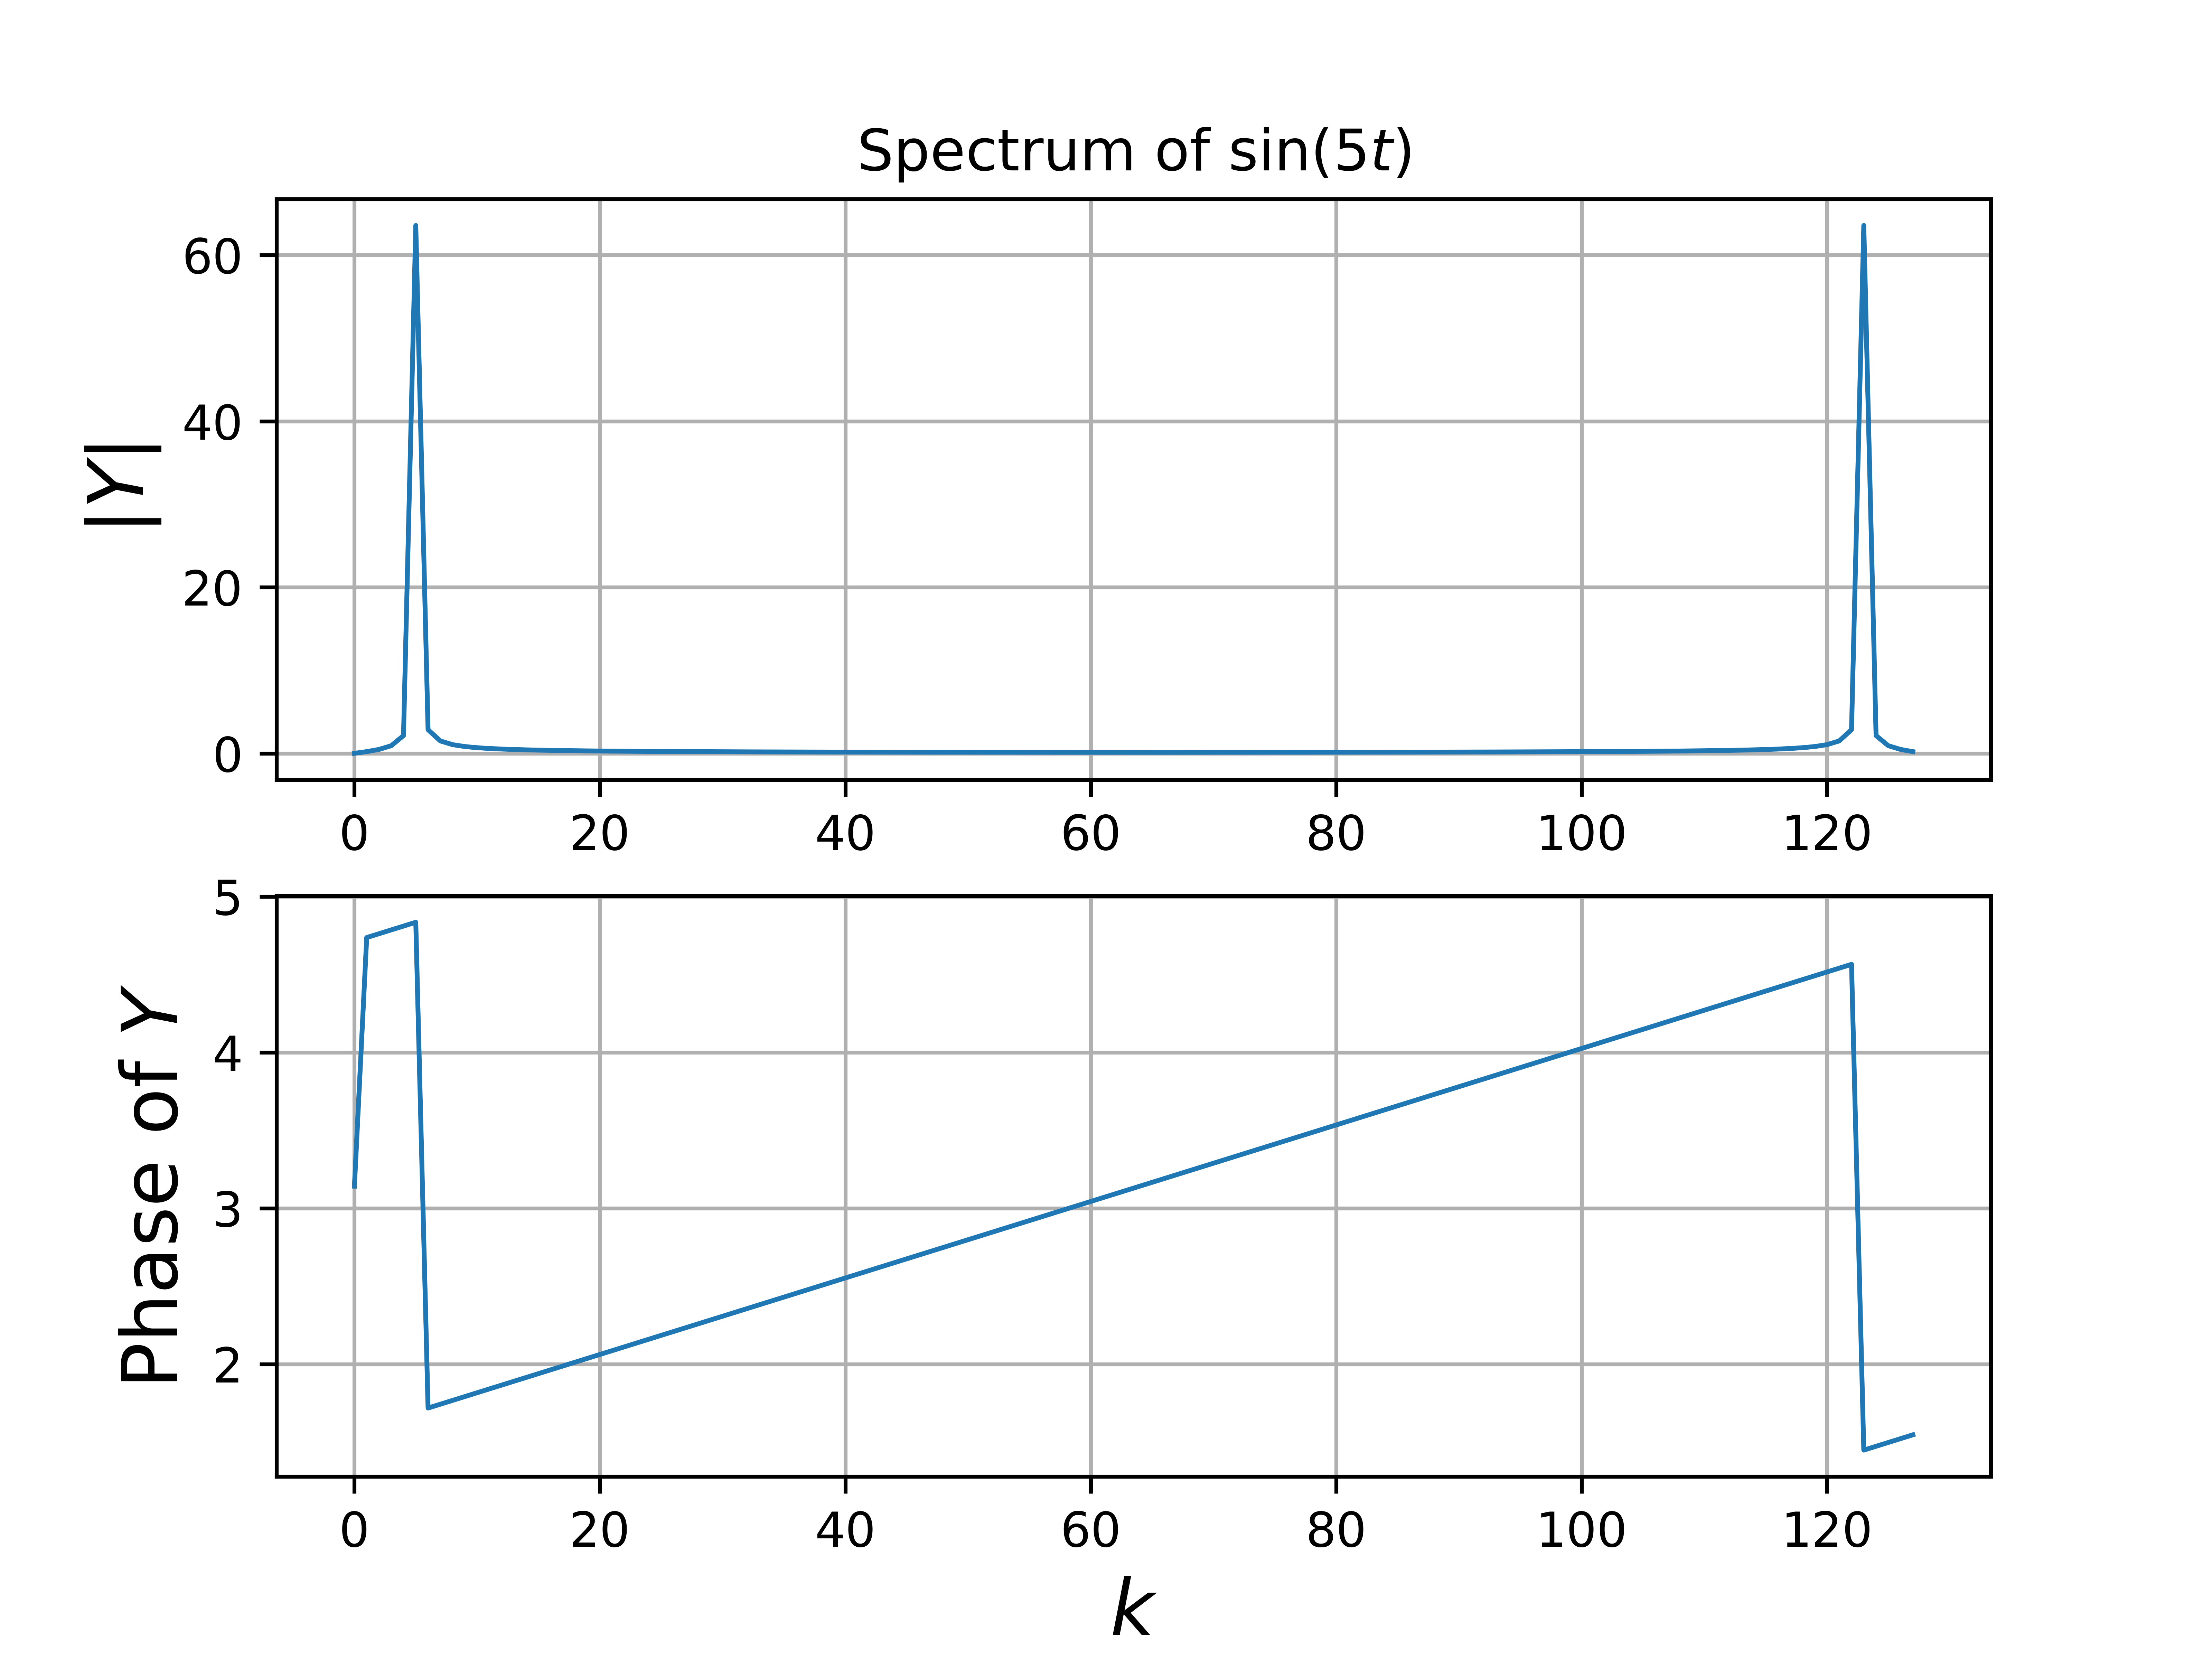
\includegraphics[scale=0.8]{images/fig0.png}
\end{center}

\subsection{Function to simplify plotting}

Now, almost all the remaining graphs require to be plotted in the same fashion, and hence I wrote a function to help me plot these:

\begin{lstlisting}[language=Python]
def plotter(function, start, end, samples, lim, title, sig=False, save=True, fignum=1):
    t = np.linspace(start,end,samples+1)[:-1]

    y = eval(function)
    Y = np.fft.fftshift(np.fft.fft(y))/samples
    maxval = samples/((end-start)//np.pi)
    w = np.linspace(-maxval,maxval,samples+1)[:-1]
    plt.figure(fignum)
    plt.subplot(2,1,1)
    plt.plot(w,abs(Y),lw=1)
    plt.xlim([-lim,lim])
    plt.ylabel(r"$|Y|$",size=16)
    plt.title(title)
    plt.grid(True)
    plt.subplot(2,1,2)
    if not sig:
        plt.plot(w,np.angle(Y),'ro',lw=1)
    ii = np.where(abs(Y)>1e-3)
    plt.plot(w[ii],np.angle(Y[ii]),'go',lw=1)
    plt.xlim([-lim,lim])
    plt.ylabel(r"Phase of $Y$",size=16)
    plt.xlabel(r"$\omega$",size=16)
    plt.grid(True)
    if save:
        plt.savefig("images/fig"+str(fignum)+".png",dpi=1000)
    plt.show()
\end{lstlisting}

In line 6 above, the logic used is that we need to ensure that the spacing and the sampling frequency correspond to real frequencies. Hence, we divide the number of samples by the number of multiples of $\pi$ in our range so that the frequencies we get correspond to real frequency values

\textbf{Explanation of this function's parameters:}
\begin{lstlisting}
    --Arguments--
    function:   a python expression for the function to be evaluated in terms of 't'
    start:      the value to start sampling at
    end:        the value to end sampling at
    samples:    the number of samples to be used for t
    lim:        the plot will be plotted between [-lim,lim]
    title:      the title of the plot in r-string form
    sig=False:  whether to plot phase points having significant phase only or all. Plots all if not specified
    save=False: boolean, saves figure as "fig"+str(fignum)+".png" if True, doesn't save if not specified
    fignum=1:   the figure number for matplotlib. Will be used to save figure if save=True

    --Example usage--
    plotter('np.sin(6*t)', -2*np.pi, 2*np.pi, 128, 10, r'Corrected Spectrum of $\sin(6t)$',True)
\end{lstlisting}

Now, using this function, it will be much easier to plot the rest of the functions.

Getting back to correcting example number 1:
\subsection{Example 1 with corrections}

To find the Fourier spectrum of $\sin(5t)$ with the peaks in the right locations.

This time, we use the helper function which takes \texttt{fftshift} and magnitude scaling into account:

\begin{lstlisting}[language=Python]
plotter("np.sin(5*t)", 0, 2*np.pi, 128, 10, r"Corrected Spectrum of $\sin(5t)$",save=True, fignum=1)
\end{lstlisting}

The graph obtained is shown below:
\begin{center}
    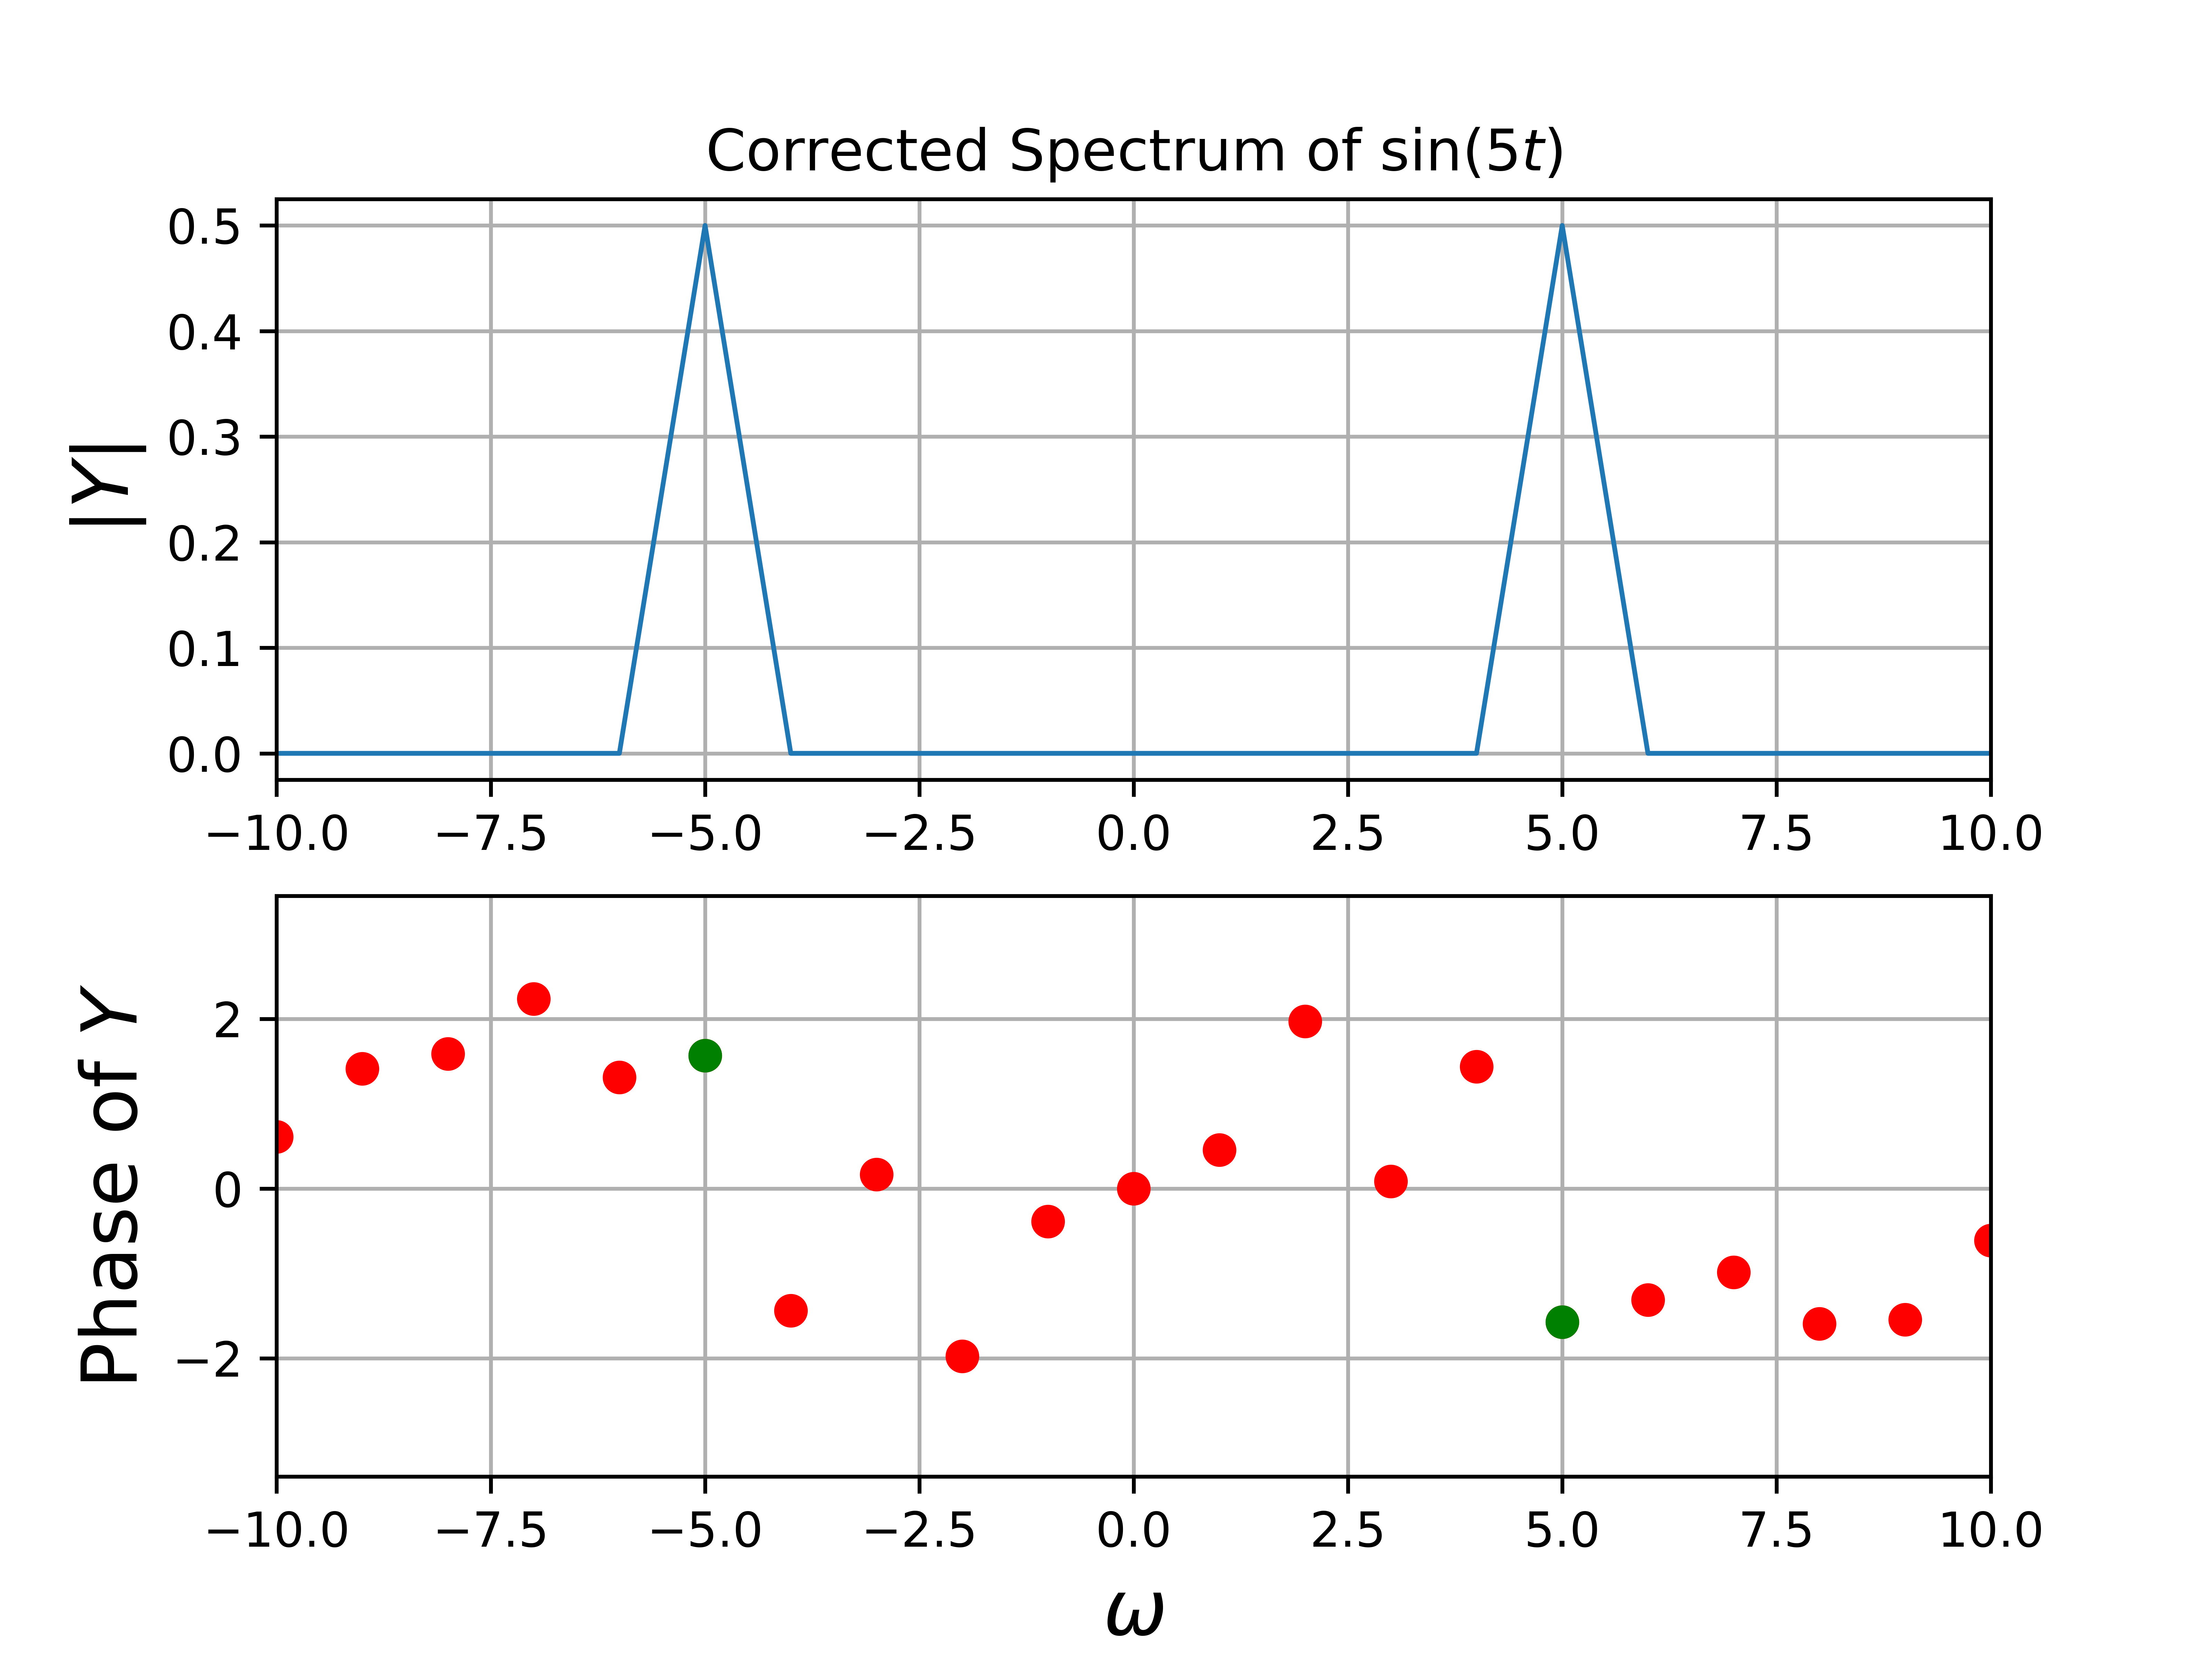
\includegraphics[scale=0.7]{images/fig1.png}
\end{center}

\subsection{Example 2}
Now we will find the Fourier Spectrum of the Amplitude Modulated Function $(1+0.1\cos(t))\cos(10t)$.

\begin{lstlisting}[language=Python]
plotter("(1 + 0.1*np.cos(t))*np.cos(10*t)",0,2*np.pi,128,15,r"Spectrum of $\left(1+0.1\cos\left(t\right)\right)\cos\left(10t\right)$",save=True,fignum=2)
\end{lstlisting}

The graph obtained is shown below:
\begin{center}
    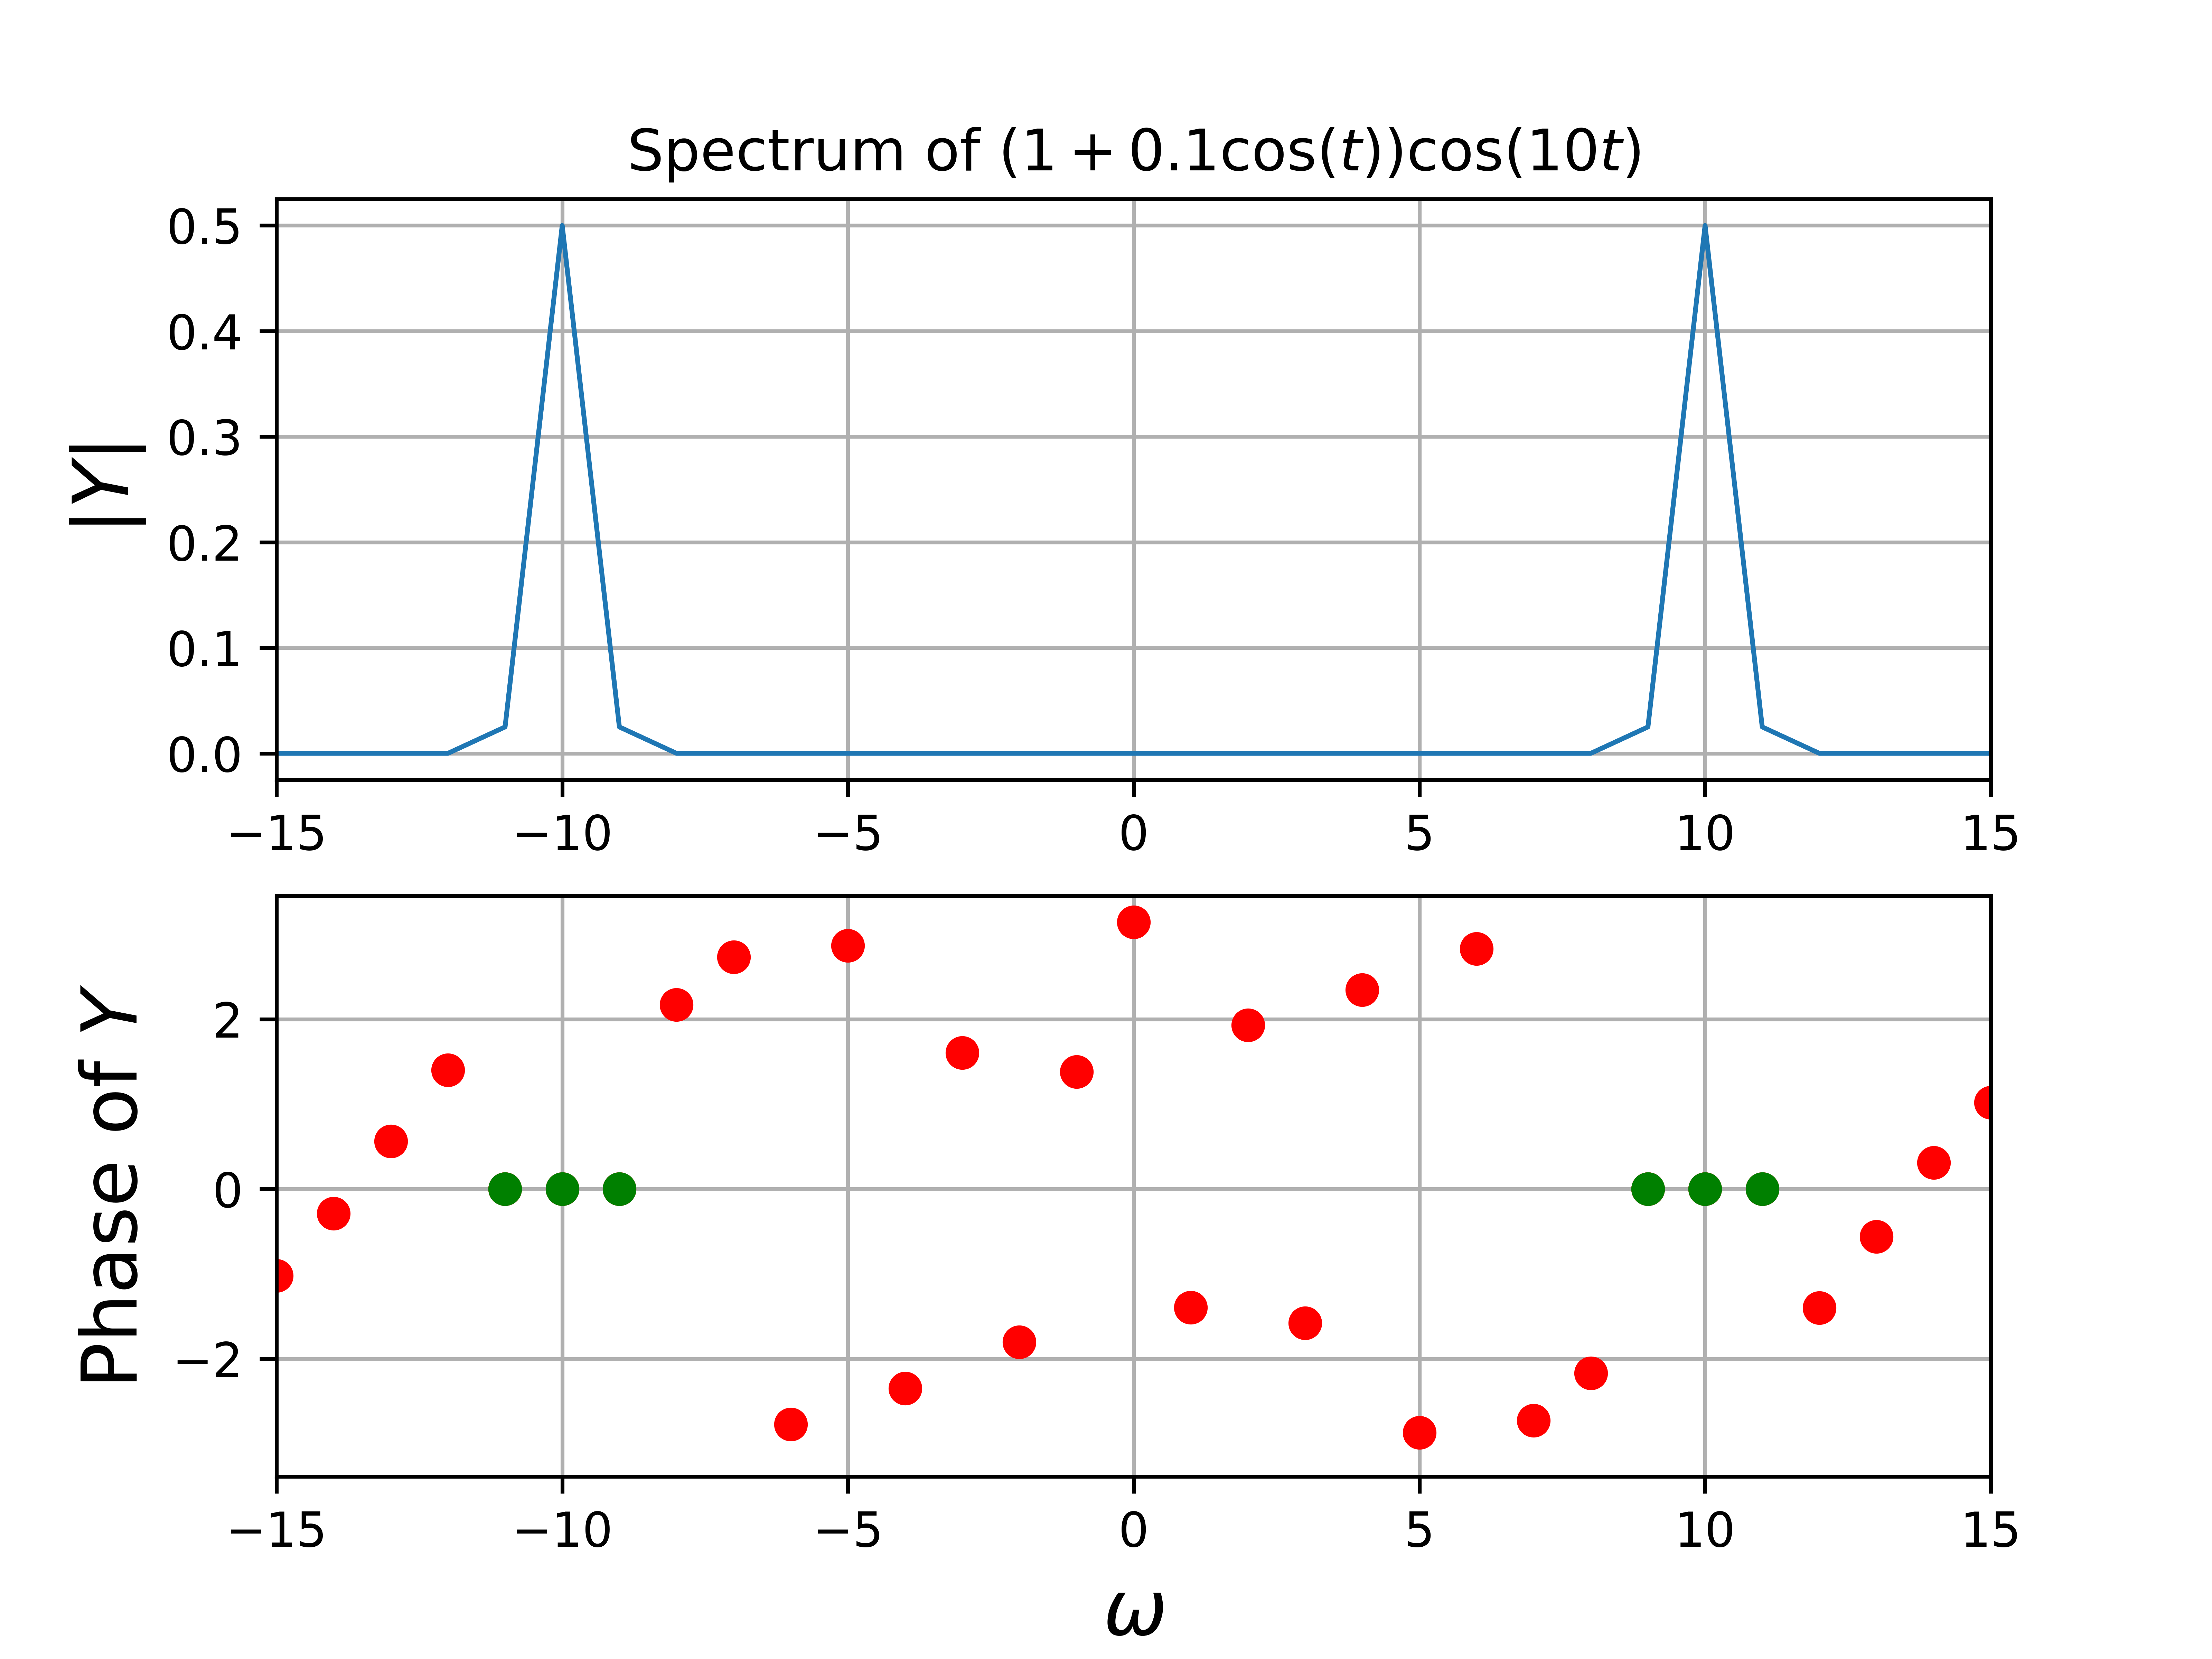
\includegraphics[scale=0.7]{images/fig2.png}
\end{center}

However, this has only 2 peaks and not 6 like it is supposed to have.

Hence, we increase the number of samples to 512 as follows:
\begin{lstlisting}[language=Python]
plotter("(1 + 0.1*np.cos(t))*np.cos(10*t)",-4*np.pi,4*np.pi,512,15,r"Spectrum of $\left(1+0.1\cos\left(t\right)\right)\cos\left(10t\right)$",save=True,fignum=2)
\end{lstlisting}

And then we plot it to get:
\begin{center}
    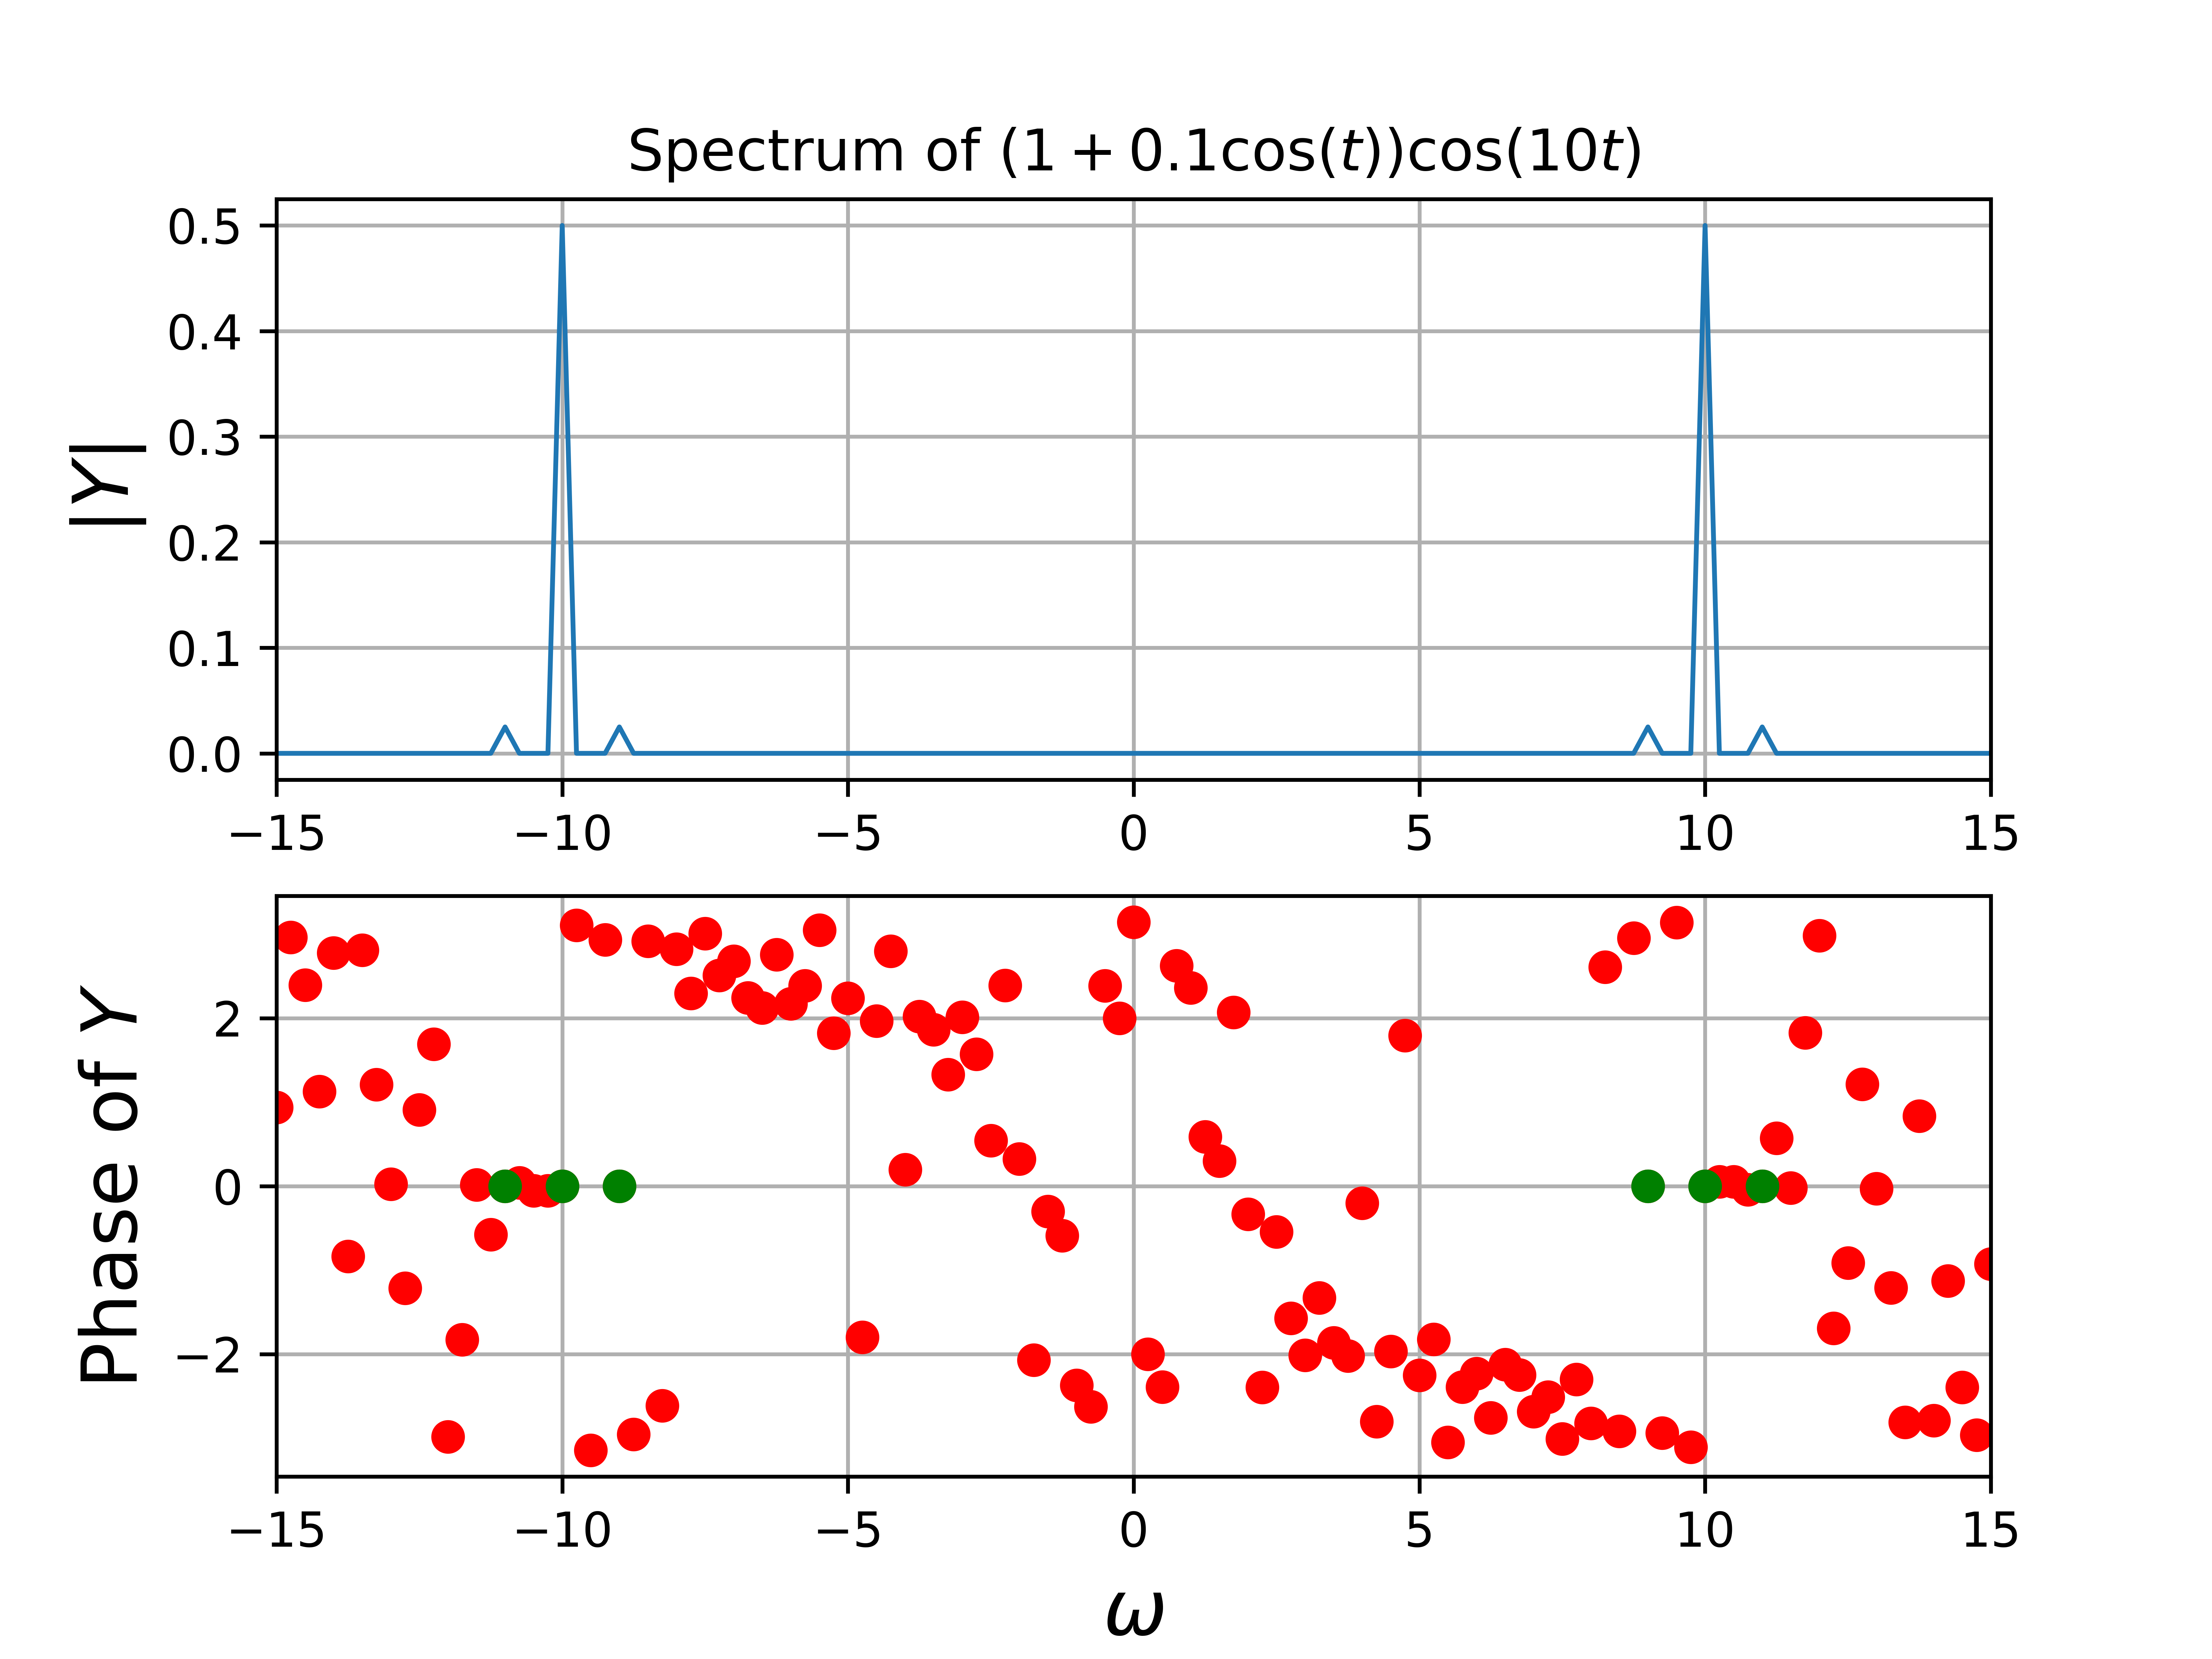
\includegraphics[scale=0.7]{images/fig3.png}
\end{center}

Now, what happens if we sample times from 0 to $8\pi$ instead?
Let's see:

\begin{lstlisting}[language=Python]
plotter("(1 + 0.1*np.cos(t))*np.cos(10*t)",0,8*np.pi,512,15,r"Spectrum of $\left(1+0.1\cos\left(t\right)\right)\cos\left(10t\right)$",save=True,fignum=2)
\end{lstlisting}

And we get:
\begin{center}
    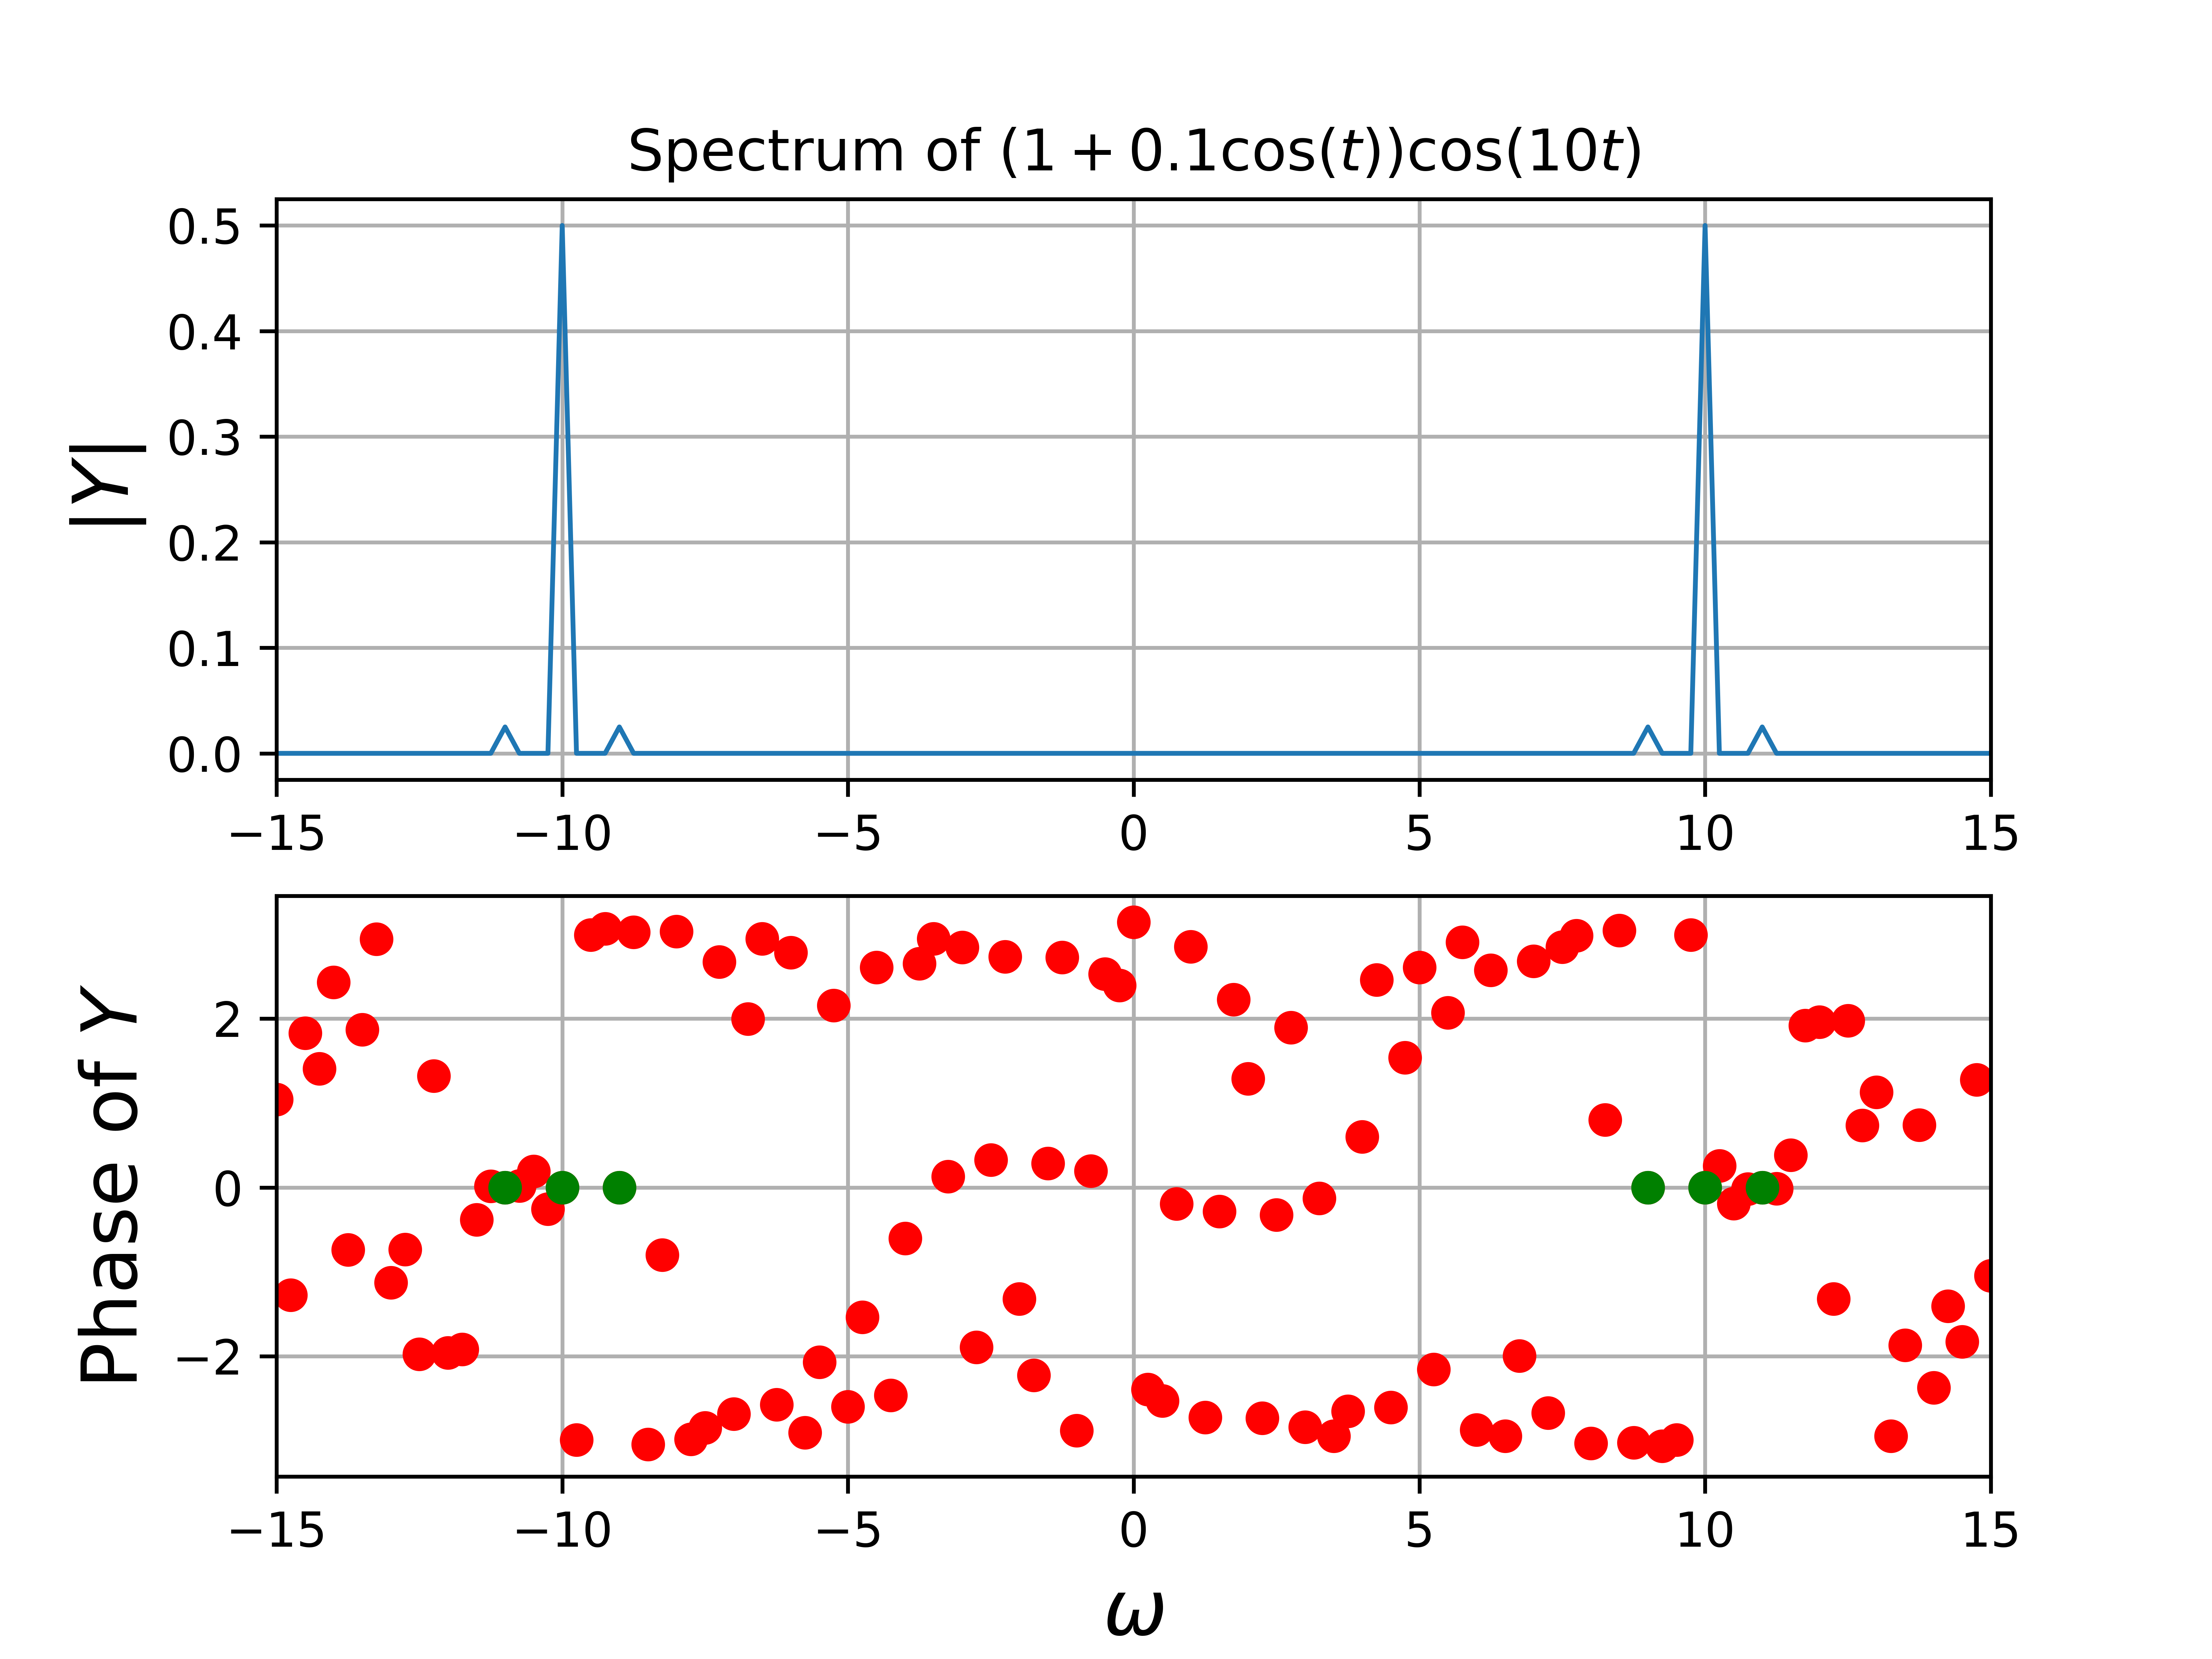
\includegraphics[scale=0.7]{images/fig4.png}
\end{center}

As we can see, there is a slight difference between the two phase plots while the magnitude plots are identical. 

This is just an error due to the small non-zero values in the imaginary part. 

Phase is undefined if magnitude is zero, hence we can safely ignore those values.
\pagebreak
\section{Question 2}

\subsection{Fourier Spectrum of $sin^3(t)$}

\textbf{Code:}
\begin{lstlisting}[language=Python]
plotter("(np.sin(t))**3",0,8*np.pi,512,4,r"Spectrum of $\sin^3(t)$",save=True,fignum=5)
\end{lstlisting}

\textbf{Expected Spectrum:}

Seeing as $sin(3t)=3sin(t)-4\sin^3(t)$, it follows $sin^3(t)=\frac{3}{4}sin(t)-\frac{1}{4}sin(3t)$ hence we should be having peaks of 0.375 at $t = \pm 1$ and peaks of 0.125 at $t = \pm 3$. 
This is exactly what we see in the magnitude spectrum.

Also, as it is in terms of sin(x), the phase spectrum is odd and is $-\frac{\pi}{2}$ at $t=-3$ and $1$ while it is $\frac{\pi}{2}$ at $t=-1$ and $3$. This is just what we see:

\textbf{Obtained Fourier Spectrum:}

\begin{center}
    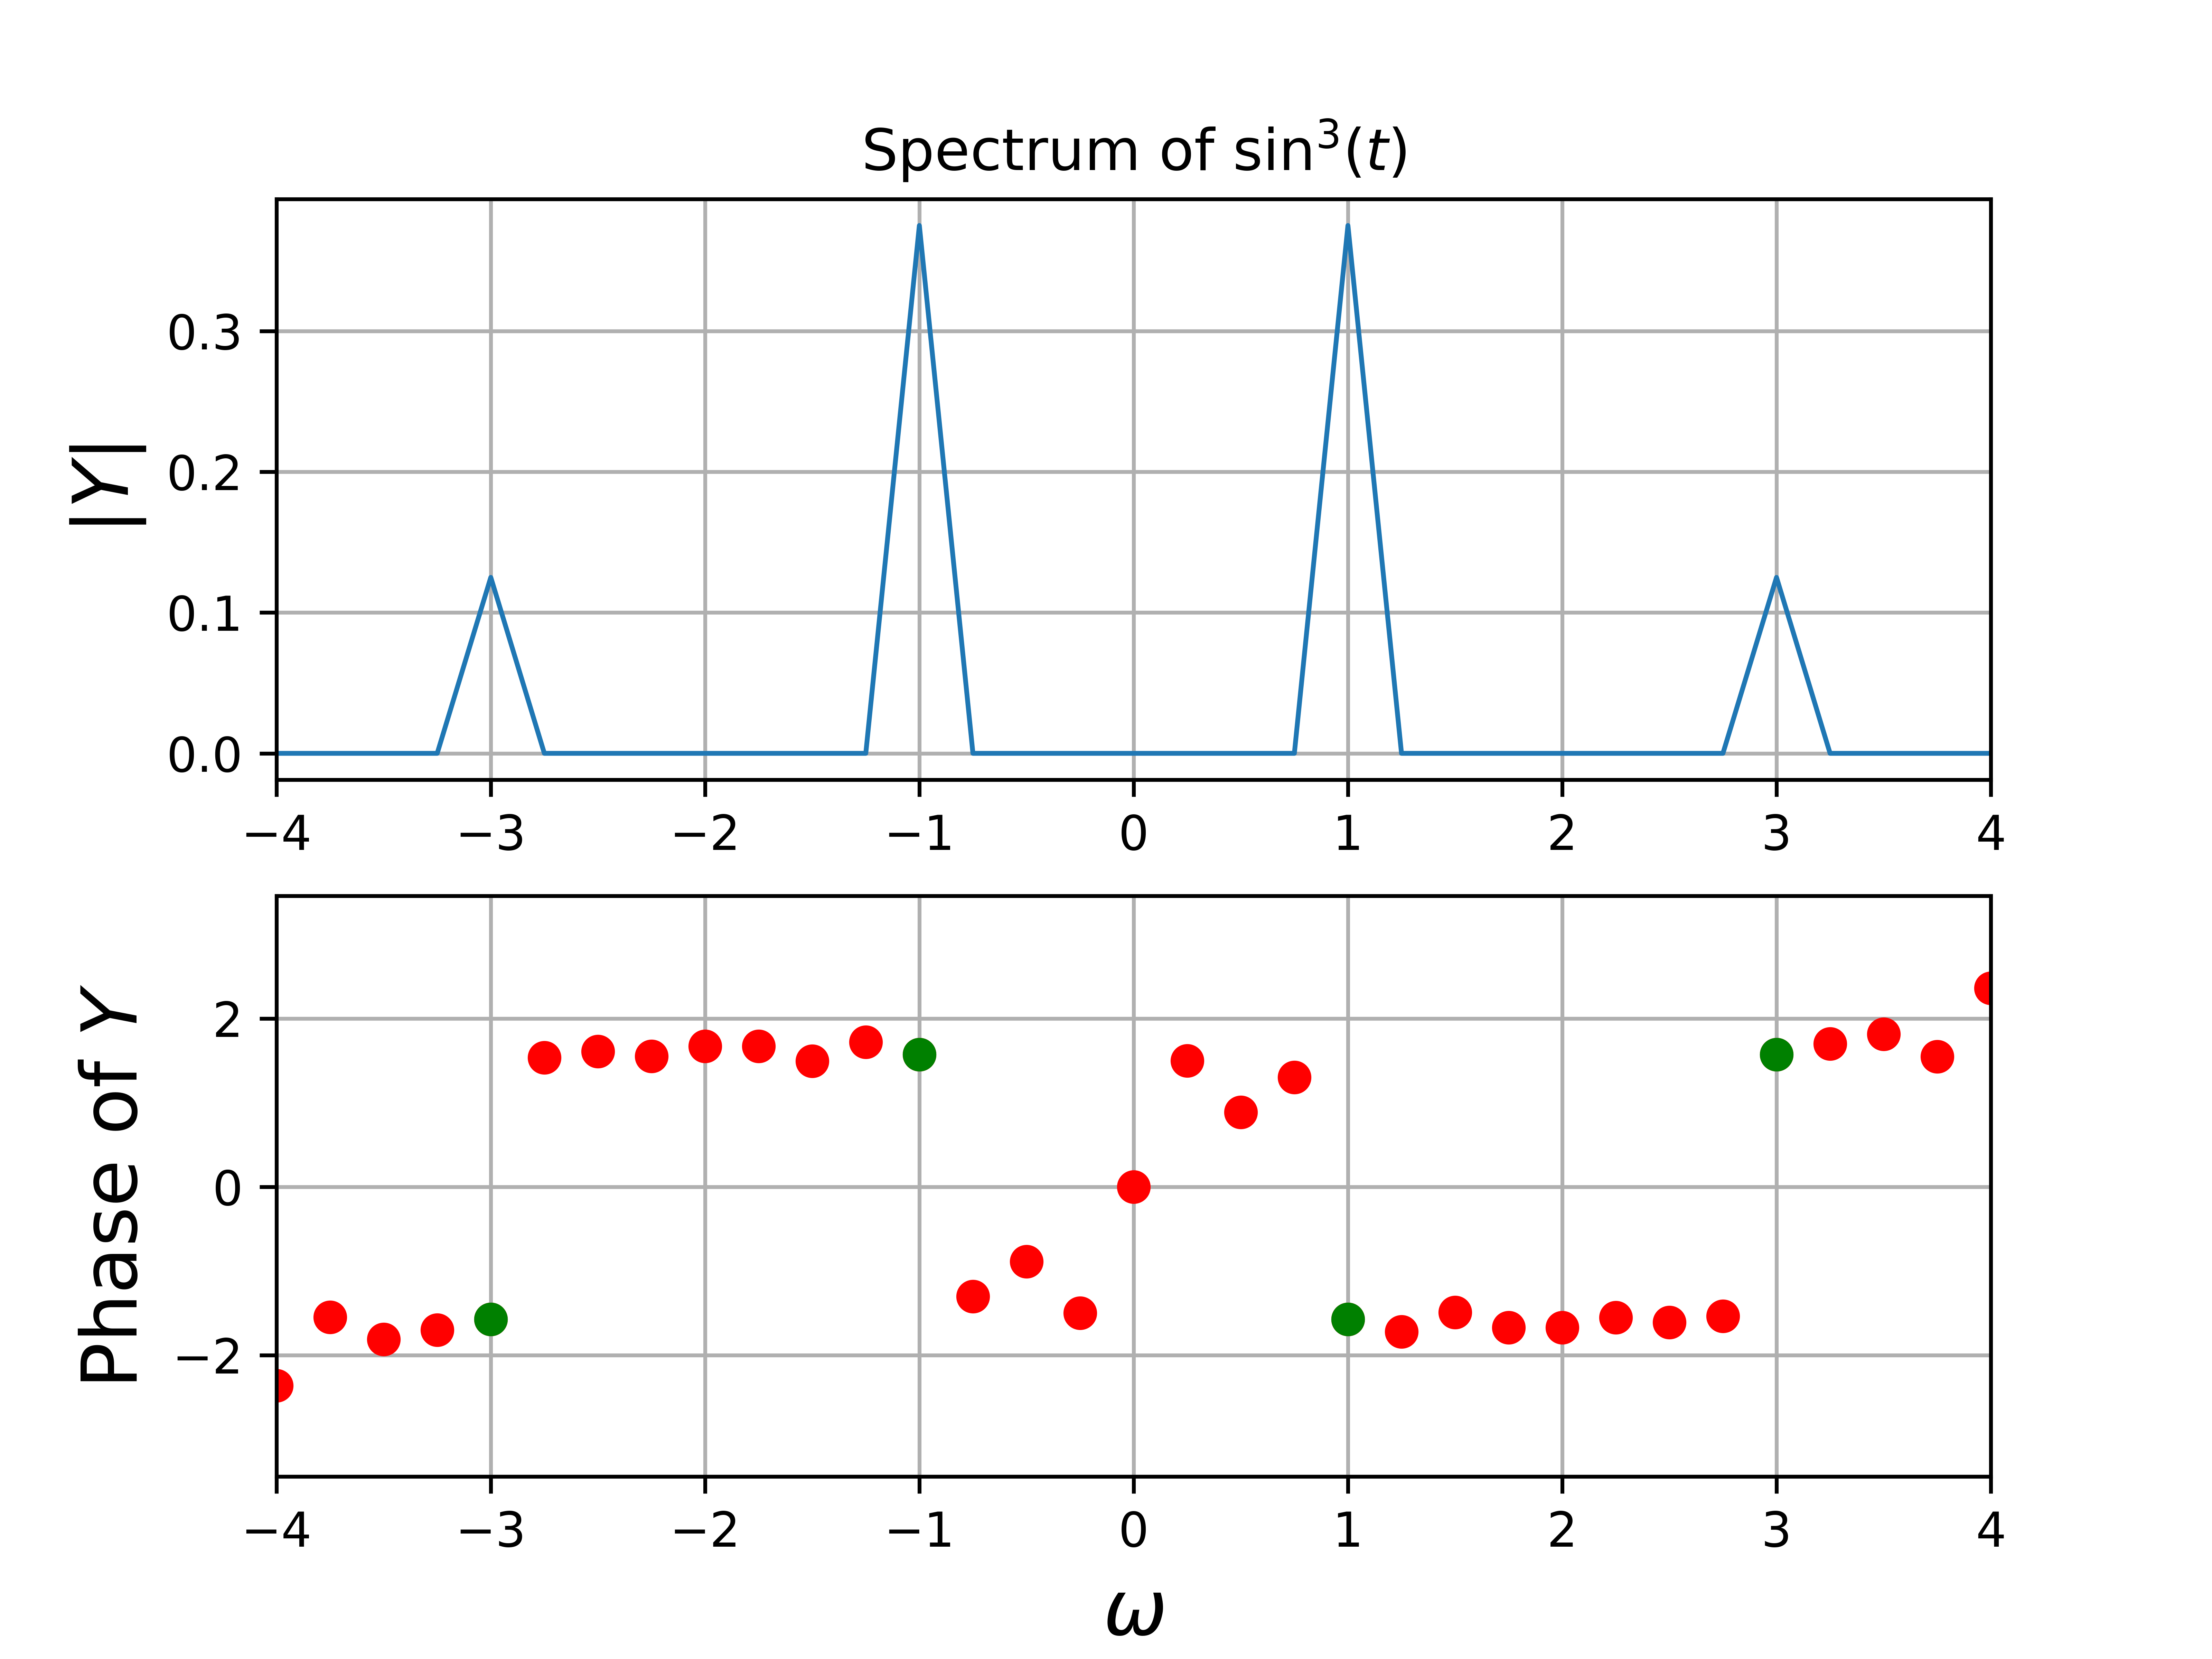
\includegraphics[scale=1]{images/fig5.png}
\end{center}

\pagebreak
\subsection{Fourier Spectrum of $cos^3(t)$}

\textbf{Code:}

\begin{lstlisting}[language=Python]
plotter("(np.cos(t))**3",0,8*np.pi,512,4,r"Spectrum of $\cos^3(t)$",save=True,fignum=6)
\end{lstlisting}

\textbf{Expected Spectrum:}

Seeing as $cos(3t)=4\cos^3(t)-3cos(t)$, it follows $cos^3(t)=\frac{3}{4}cos(t)+\frac{1}{4}cos(3t)$ hence we should be having peaks of 0.375 at $t = \pm 1$ and peaks of 0.125 at $t = \pm 3$. 
This is exactly what we see in the magnitude spectrum once again:

Also, as it is in terms of cos(t), the phase spectrum is 0 everywhere. This is just what we see as well:

\textbf{Obtained Fourier Spectrum:}

\begin{center}
    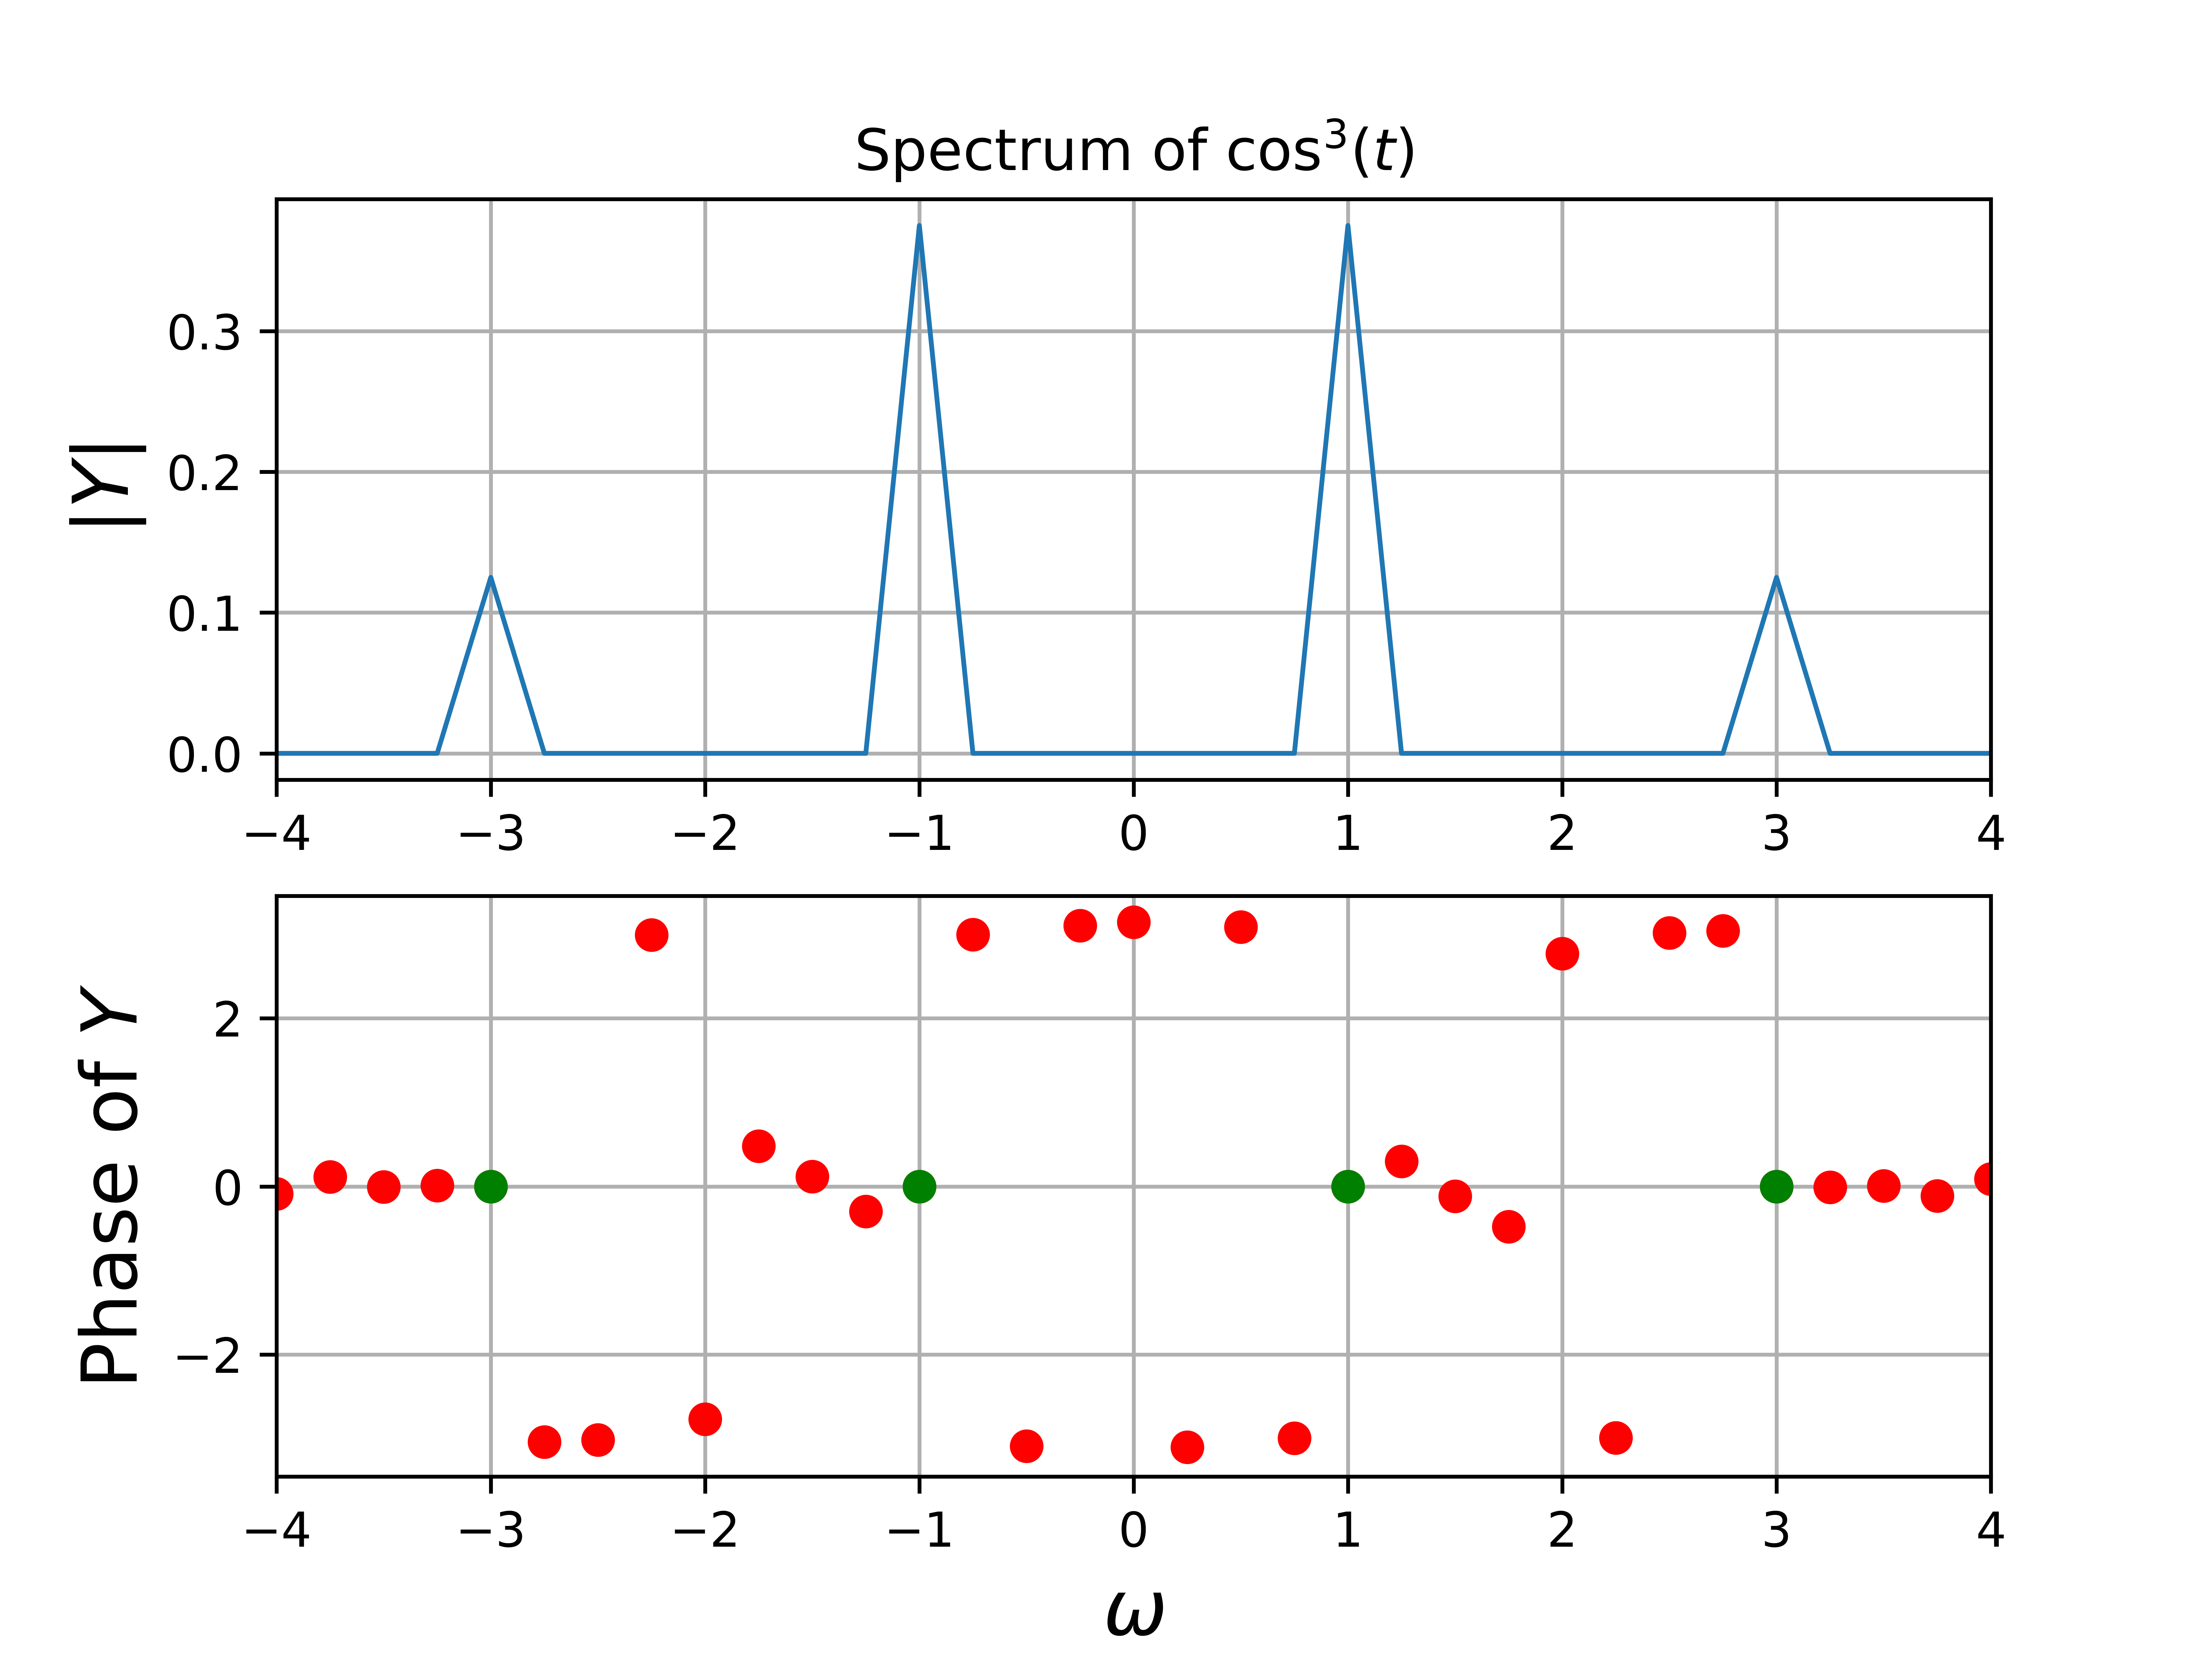
\includegraphics[scale=1]{images/fig6.png}
\end{center}
\pagebreak
\section{Question 3}
\subsection{Spectrum of $\cos(20t + 5\cos(t))$}
Only significant points will be shown in the phase plot

\textbf{Code:}

\begin{lstlisting}[language=Python]
plotter("np.cos(20*t + 5*np.cos(t))",0,8*np.pi,512,40,r"Spectrum of $\cos(20t + 5\cos(t))$",sig=True,save=True,fignum=7)
\end{lstlisting}

\textbf{Obtained Fourier Spectrum:}
\begin{center}
    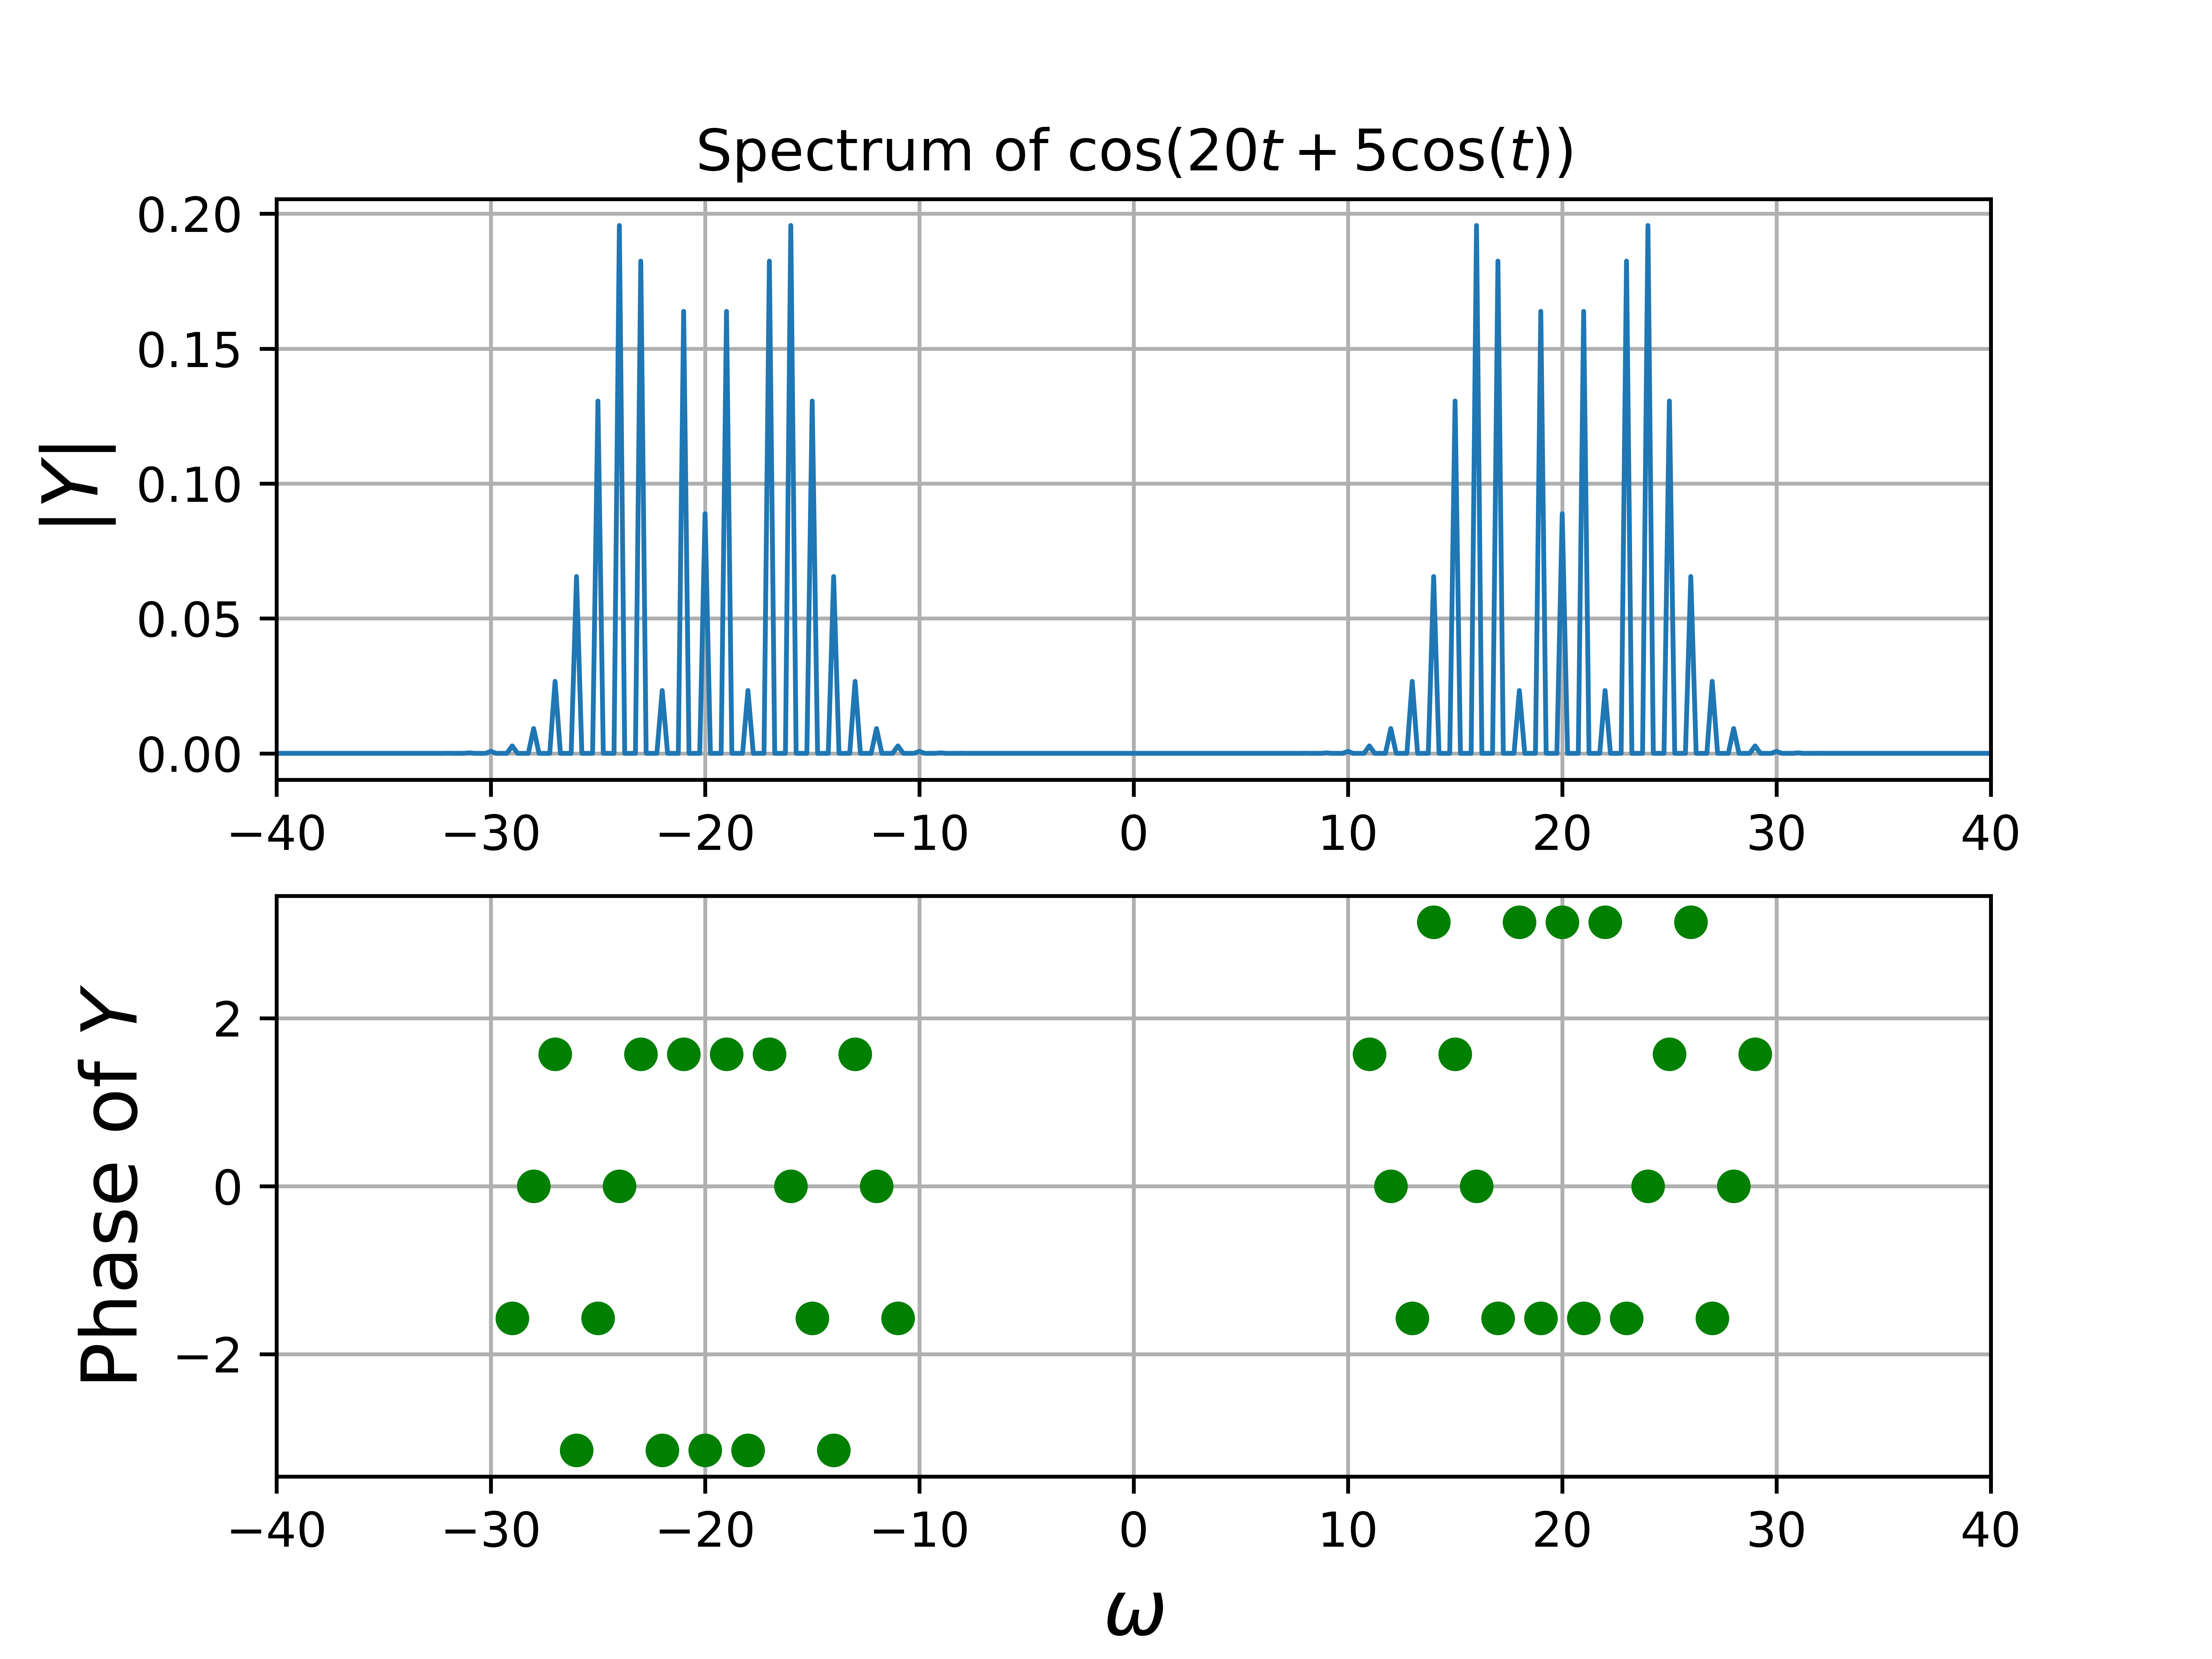
\includegraphics[scale=1]{images/fig7.png}
\end{center}
This plot looks really interesting.

\textbf{Explanation of Observed Spectrum:}

A very simplified explanation for this is that since we have a $+5\cos(t)$ term internally, it adds some extra frequencies near 20 to the Fourier Transform which dies out as we move away from 20 on either side.

The phase plot also confirms this, in a way, as we can see that at the frequencies where the magnitude is significant, the phases oscillate quickly around 20 between $\frac{\pi}{2}$ and $\pi$ on the right side, and between $\pi$ and $-\frac{\pi}{2}$ on the left and then the rate of oscillation decreases as we move away from 20

Now, a more \textbf{technical explanation}:

This is a frequency modulated wave. And, since the argument of the cosine wave itself contains a cosine, it can be expressed using Bessel functions.

When it is expressed in terms of Bessel functions, we find that there are multiple impulses at the carrier frequency  of 20 rad/s as well as many surrounding the carrier frequency.

\section{Question 4}

We are finding the DFT of the function:

$$f(t) = e^{\frac{-t^2}{2}}$$

If we take the CFT of this, we find it to be:

$$F(\omega) = \sqrt{2*\pi}e^{\frac{-\omega^2}{2}}$$

Thus, ideally, its phase must be zero and its magnitude is also a Gaussian with value $\sqrt{2*\pi}$ at $\omega=0$.

However, there are multiple caveats and pitfalls that we need to look into:

\subsection{Pitfalls}

I made multiple of these errors while coming up with this function and I'm mentioning them here for the benefit of anyone who may come upon this while learning how to use the NumPy DFT functions.

First, I sampled time from $[0,8\pi)$.

\begin{lstlisting}[language=Python]
plotter("np.exp(-(t**2)/2)",0,8*np.pi,512,50,r"Spectrum of a Gaussian $\exp(\frac{-t^2}{2})$",sig=False,save=True,fignum=8)
\end{lstlisting}

However, since this function is not periodic, if we try to plot this over this asymmetric time range, our phase spectrum comes out to be completely wrong, and non-zero:

\begin{center}
    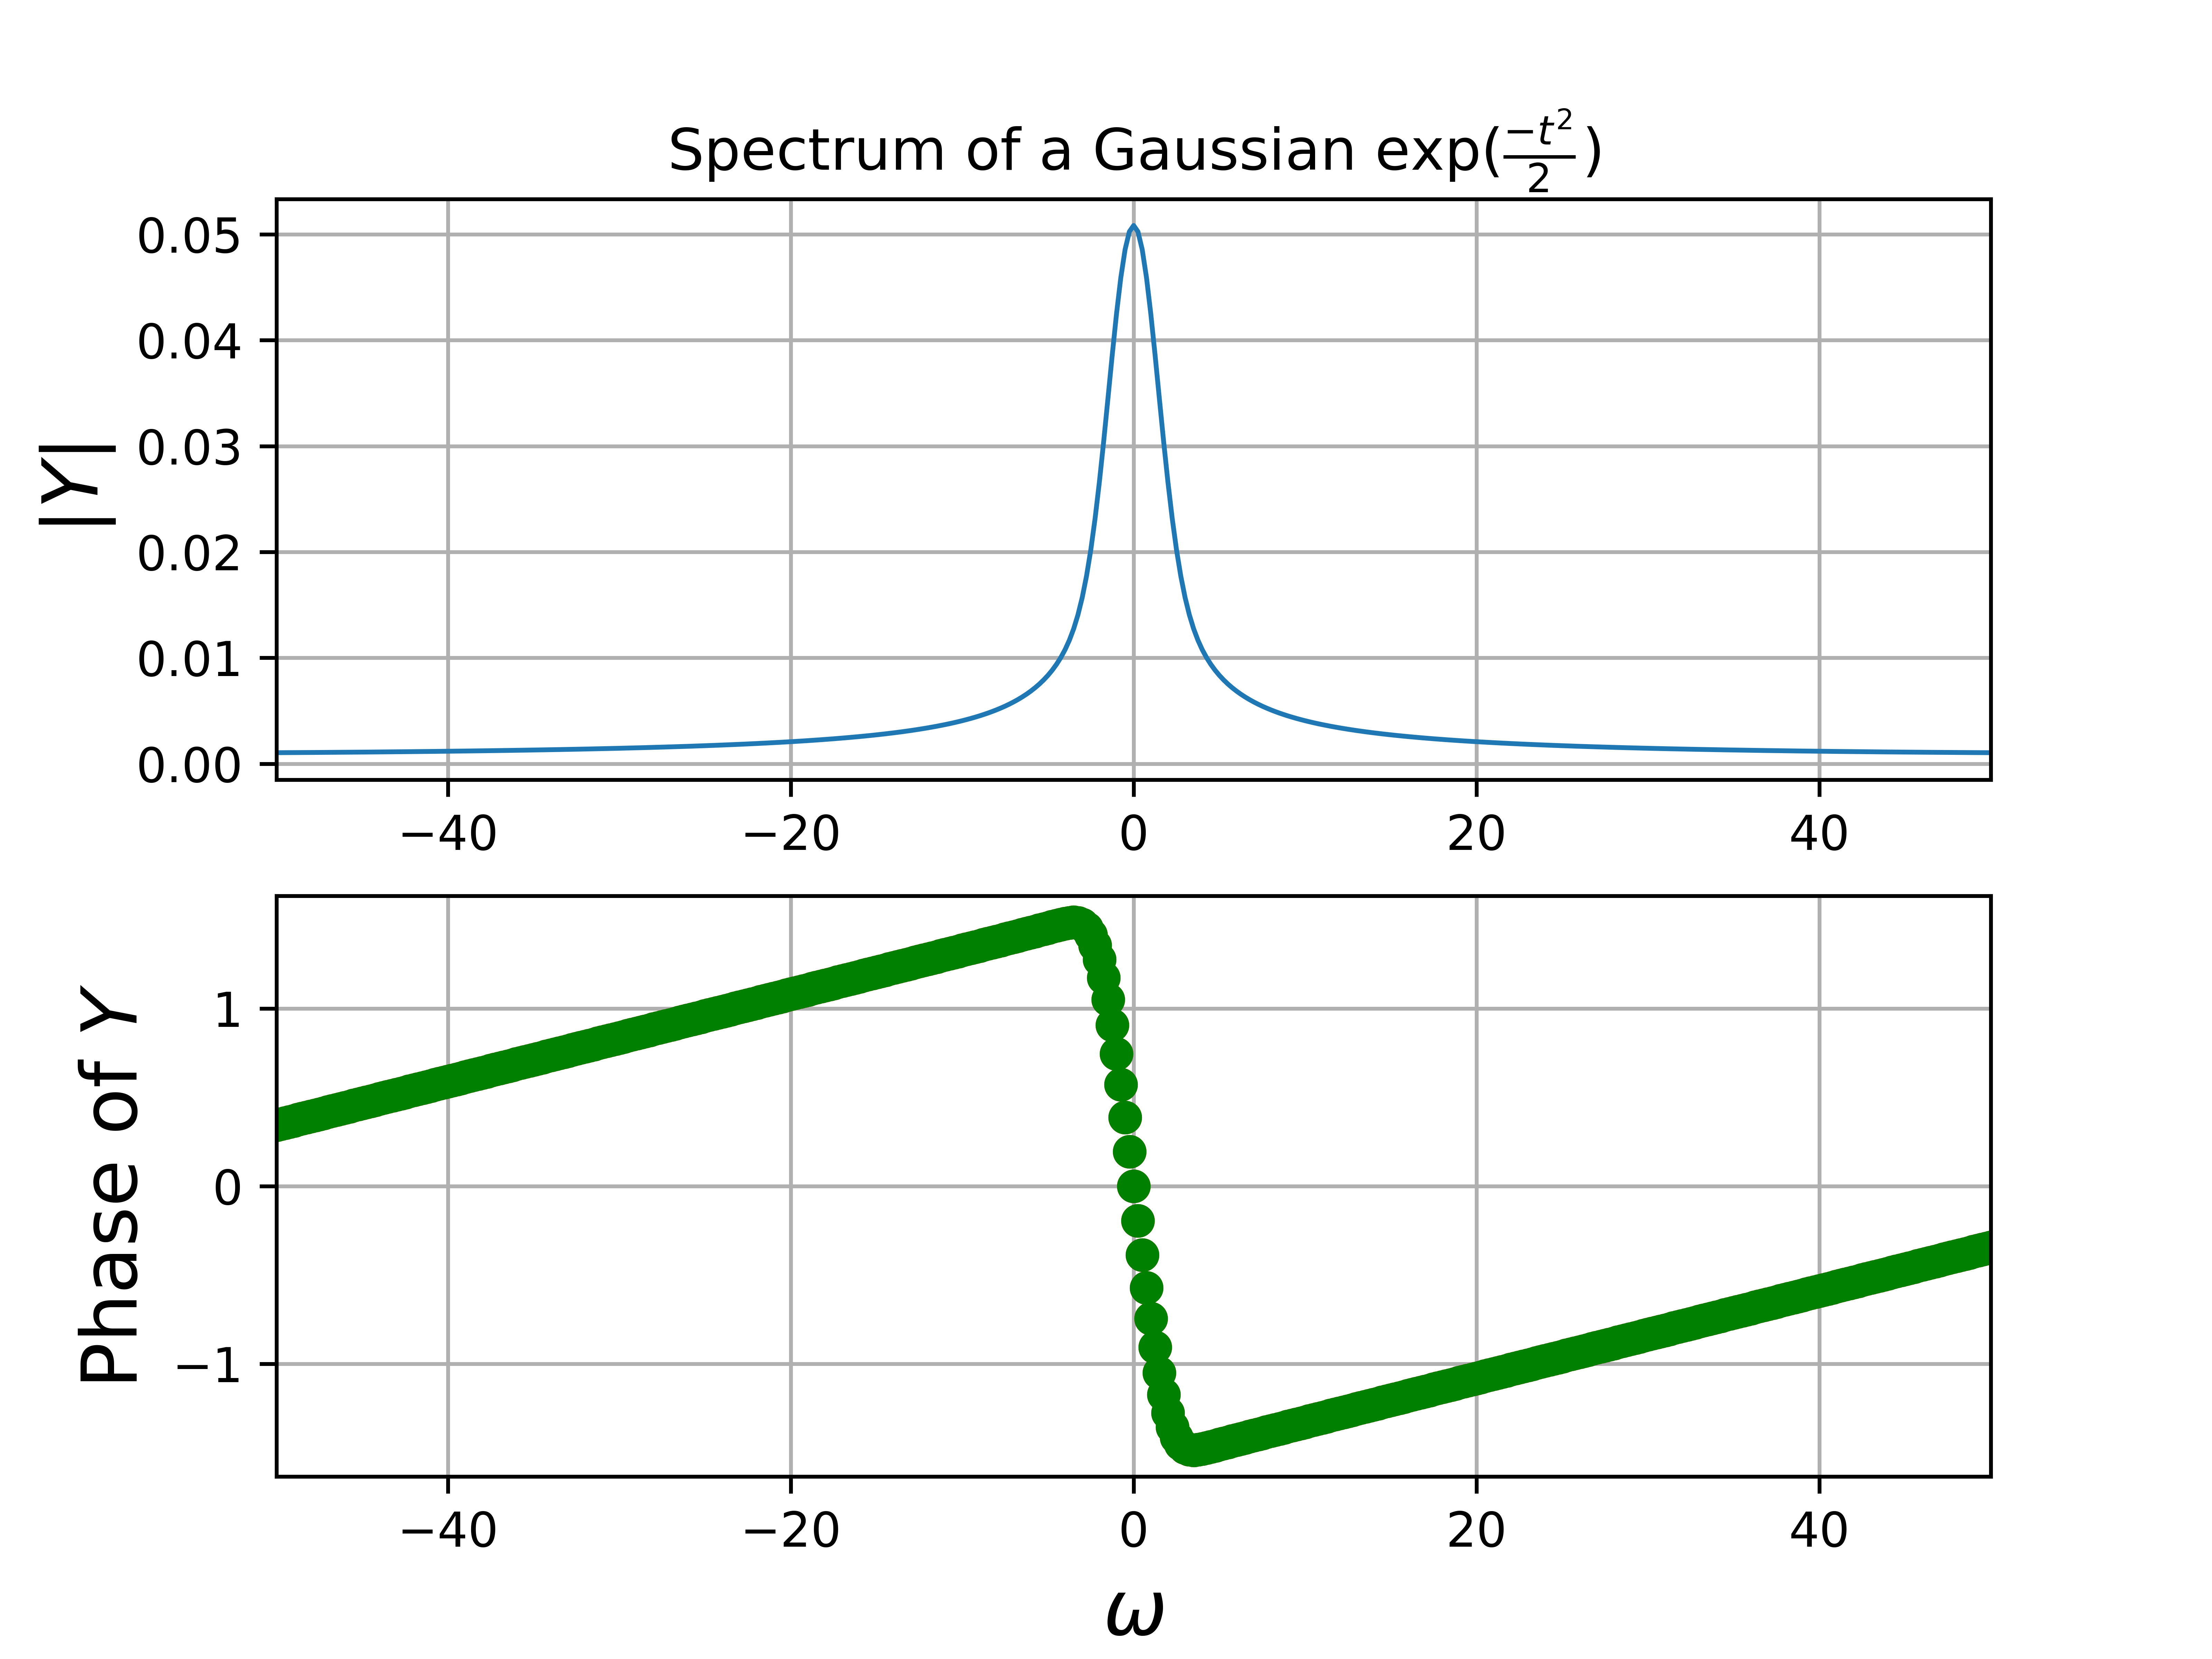
\includegraphics[scale=1]{images/fig8.png}
\end{center}

Next, I tried to directly plot this by increasing the number of samples, which again led to about half the phases being 0 and the other half being $\pi$ due to a tiny asymmetric nature of the samples that I used.

\begin{lstlisting}[language=Python]
plotter("np.exp(-(t**2)/2)",-8*np.pi,8*np.pi,1024,50,r"Spectrum of a Gaussian $\exp(\frac{-t^2}{2})$",sig=False,save=True,fignum=8)
\end{lstlisting}

\begin{center}
    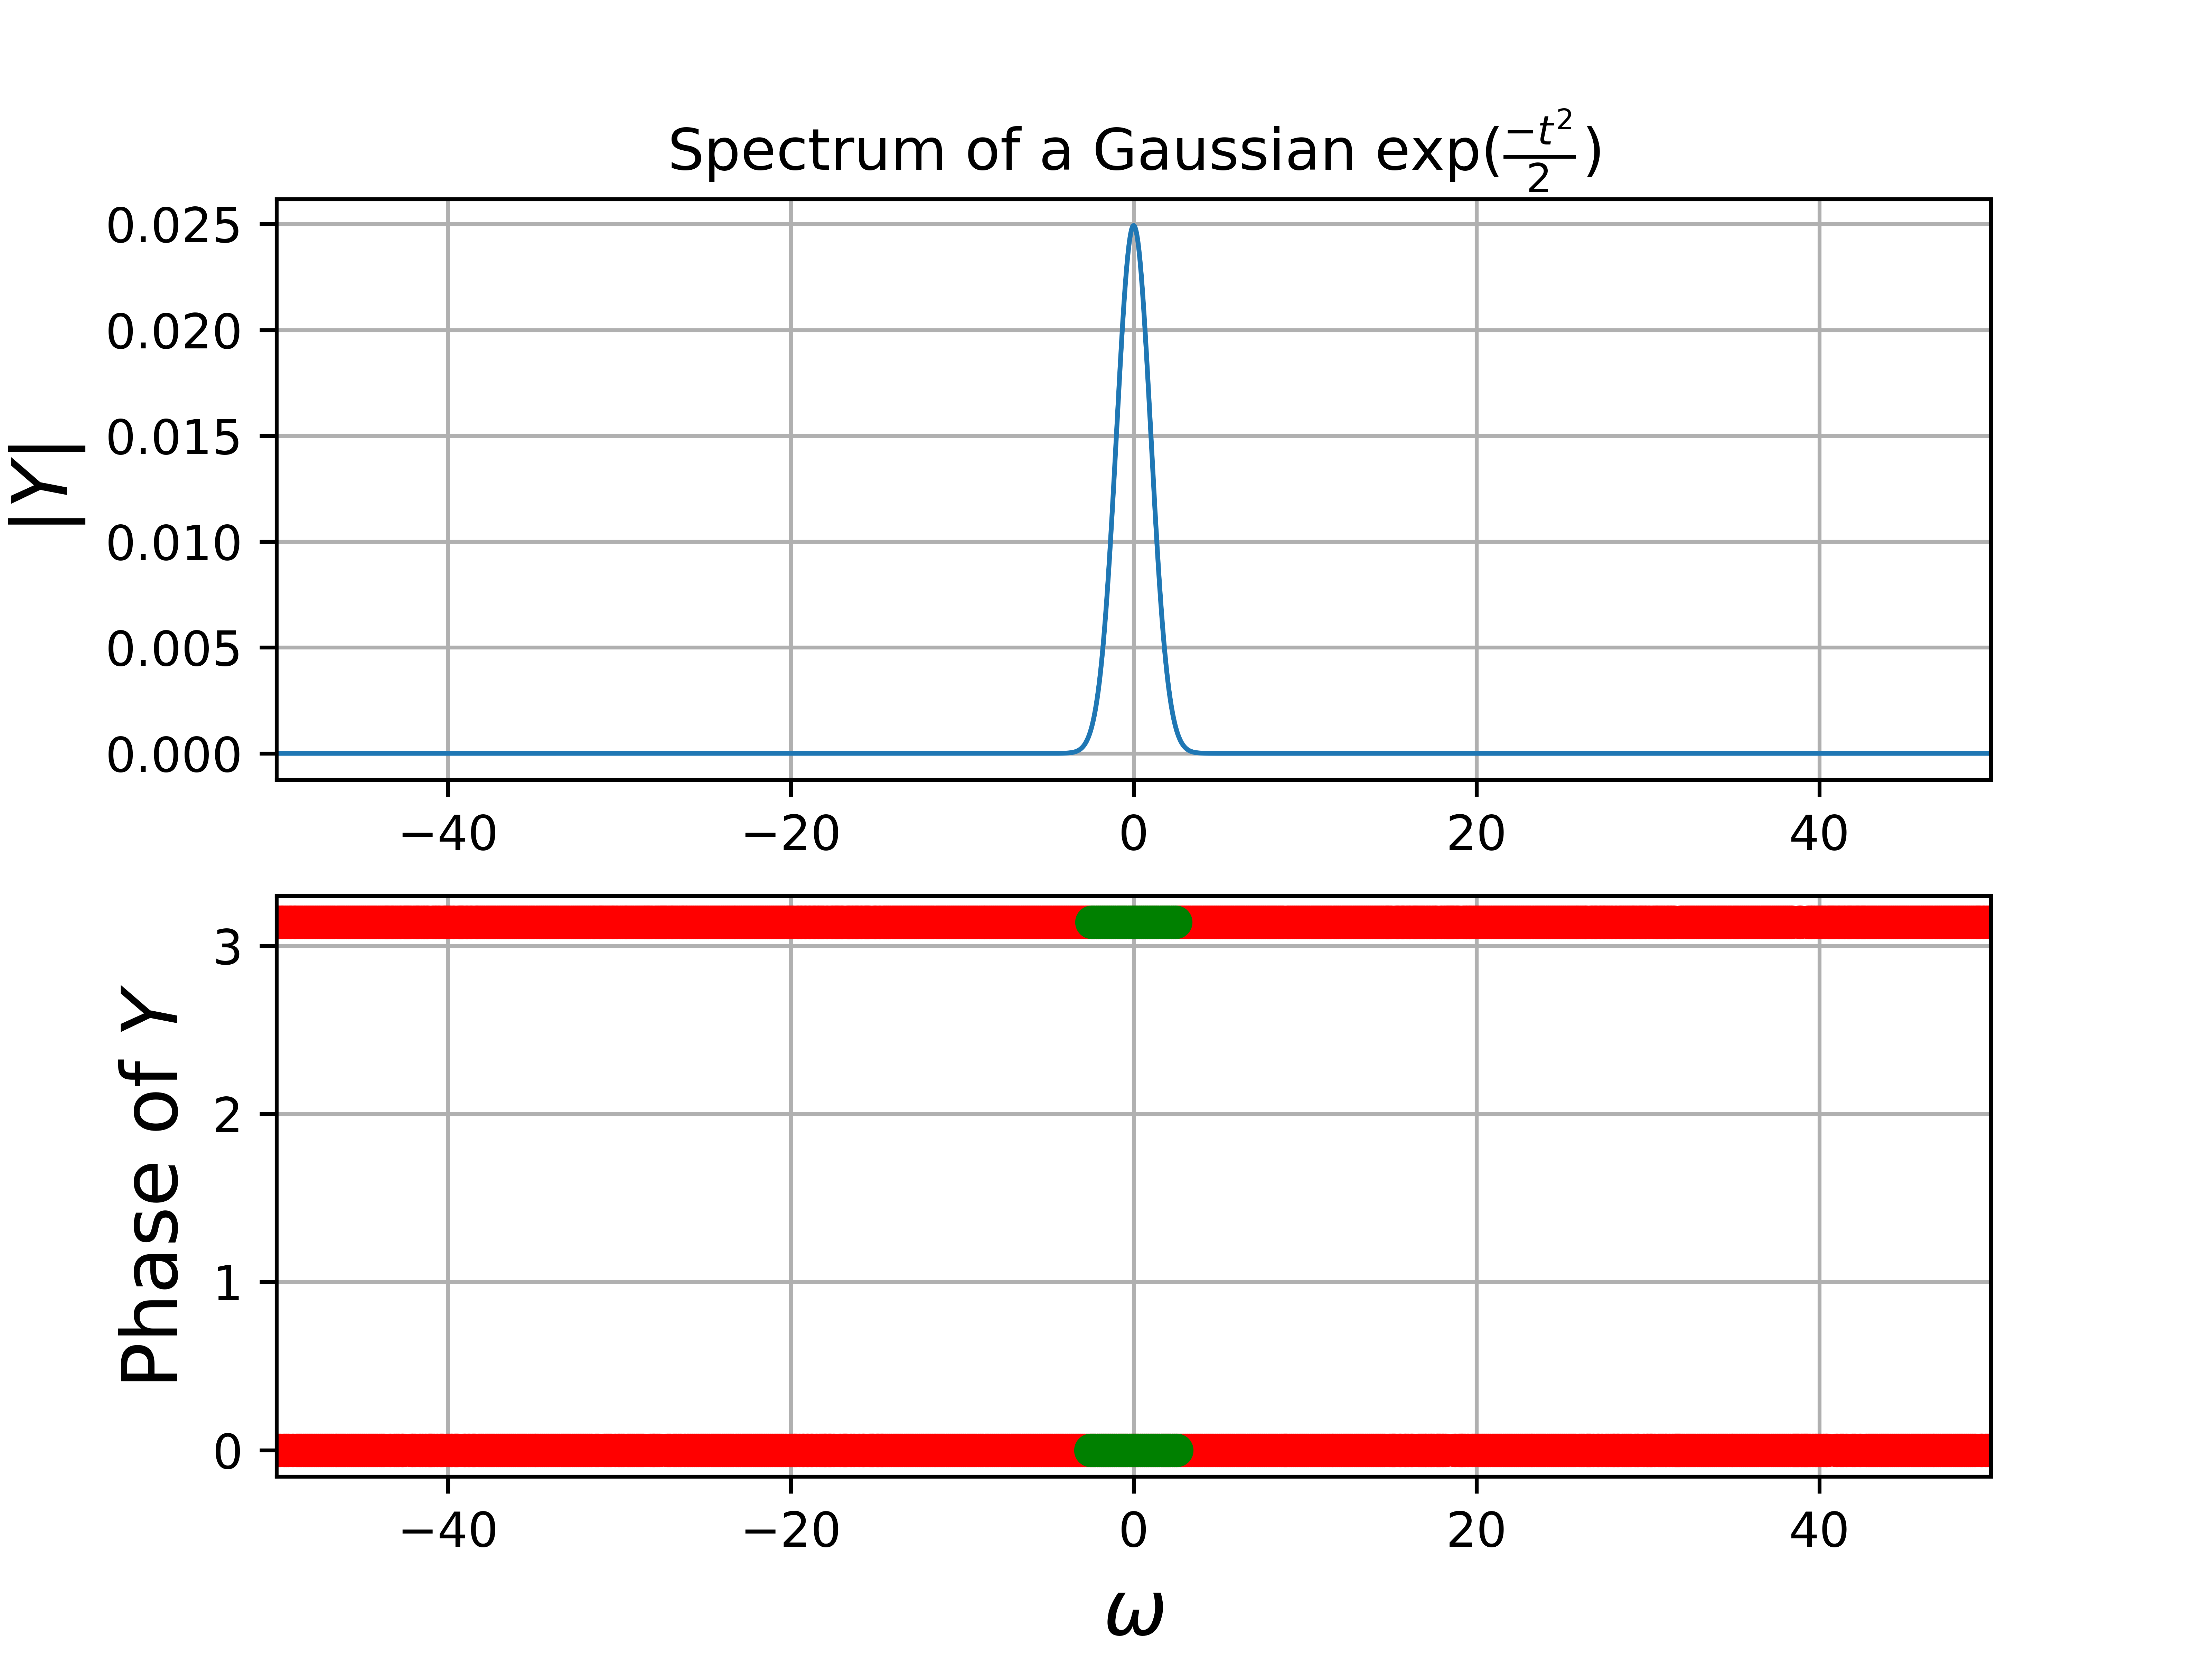
\includegraphics[scale=1]{images/fig11.png}
\end{center}

This happened because \texttt{np.linspace(-2*np.pi,2*np.pi,513)[:-1]}
is not centered at 0.

(My source and reference, although this seems trivial now: https://in.mathworks.com/matlabcentral/answers/40257-gaussian-fft)


\subsection{The Correct Way to fix everything}

It turns out that no matter how many samples you take or how closely you try to make the input centered at 0, this function is much too stubborn. Negative values keep arising no matter what.
\pagebreak
Here are some attempts:

\begin{center}
    {With time sampled over $[-65536\pi,65536\pi)$ and 4194305 samples, this took over 10 minutes to plot and render on my laptop}
    
    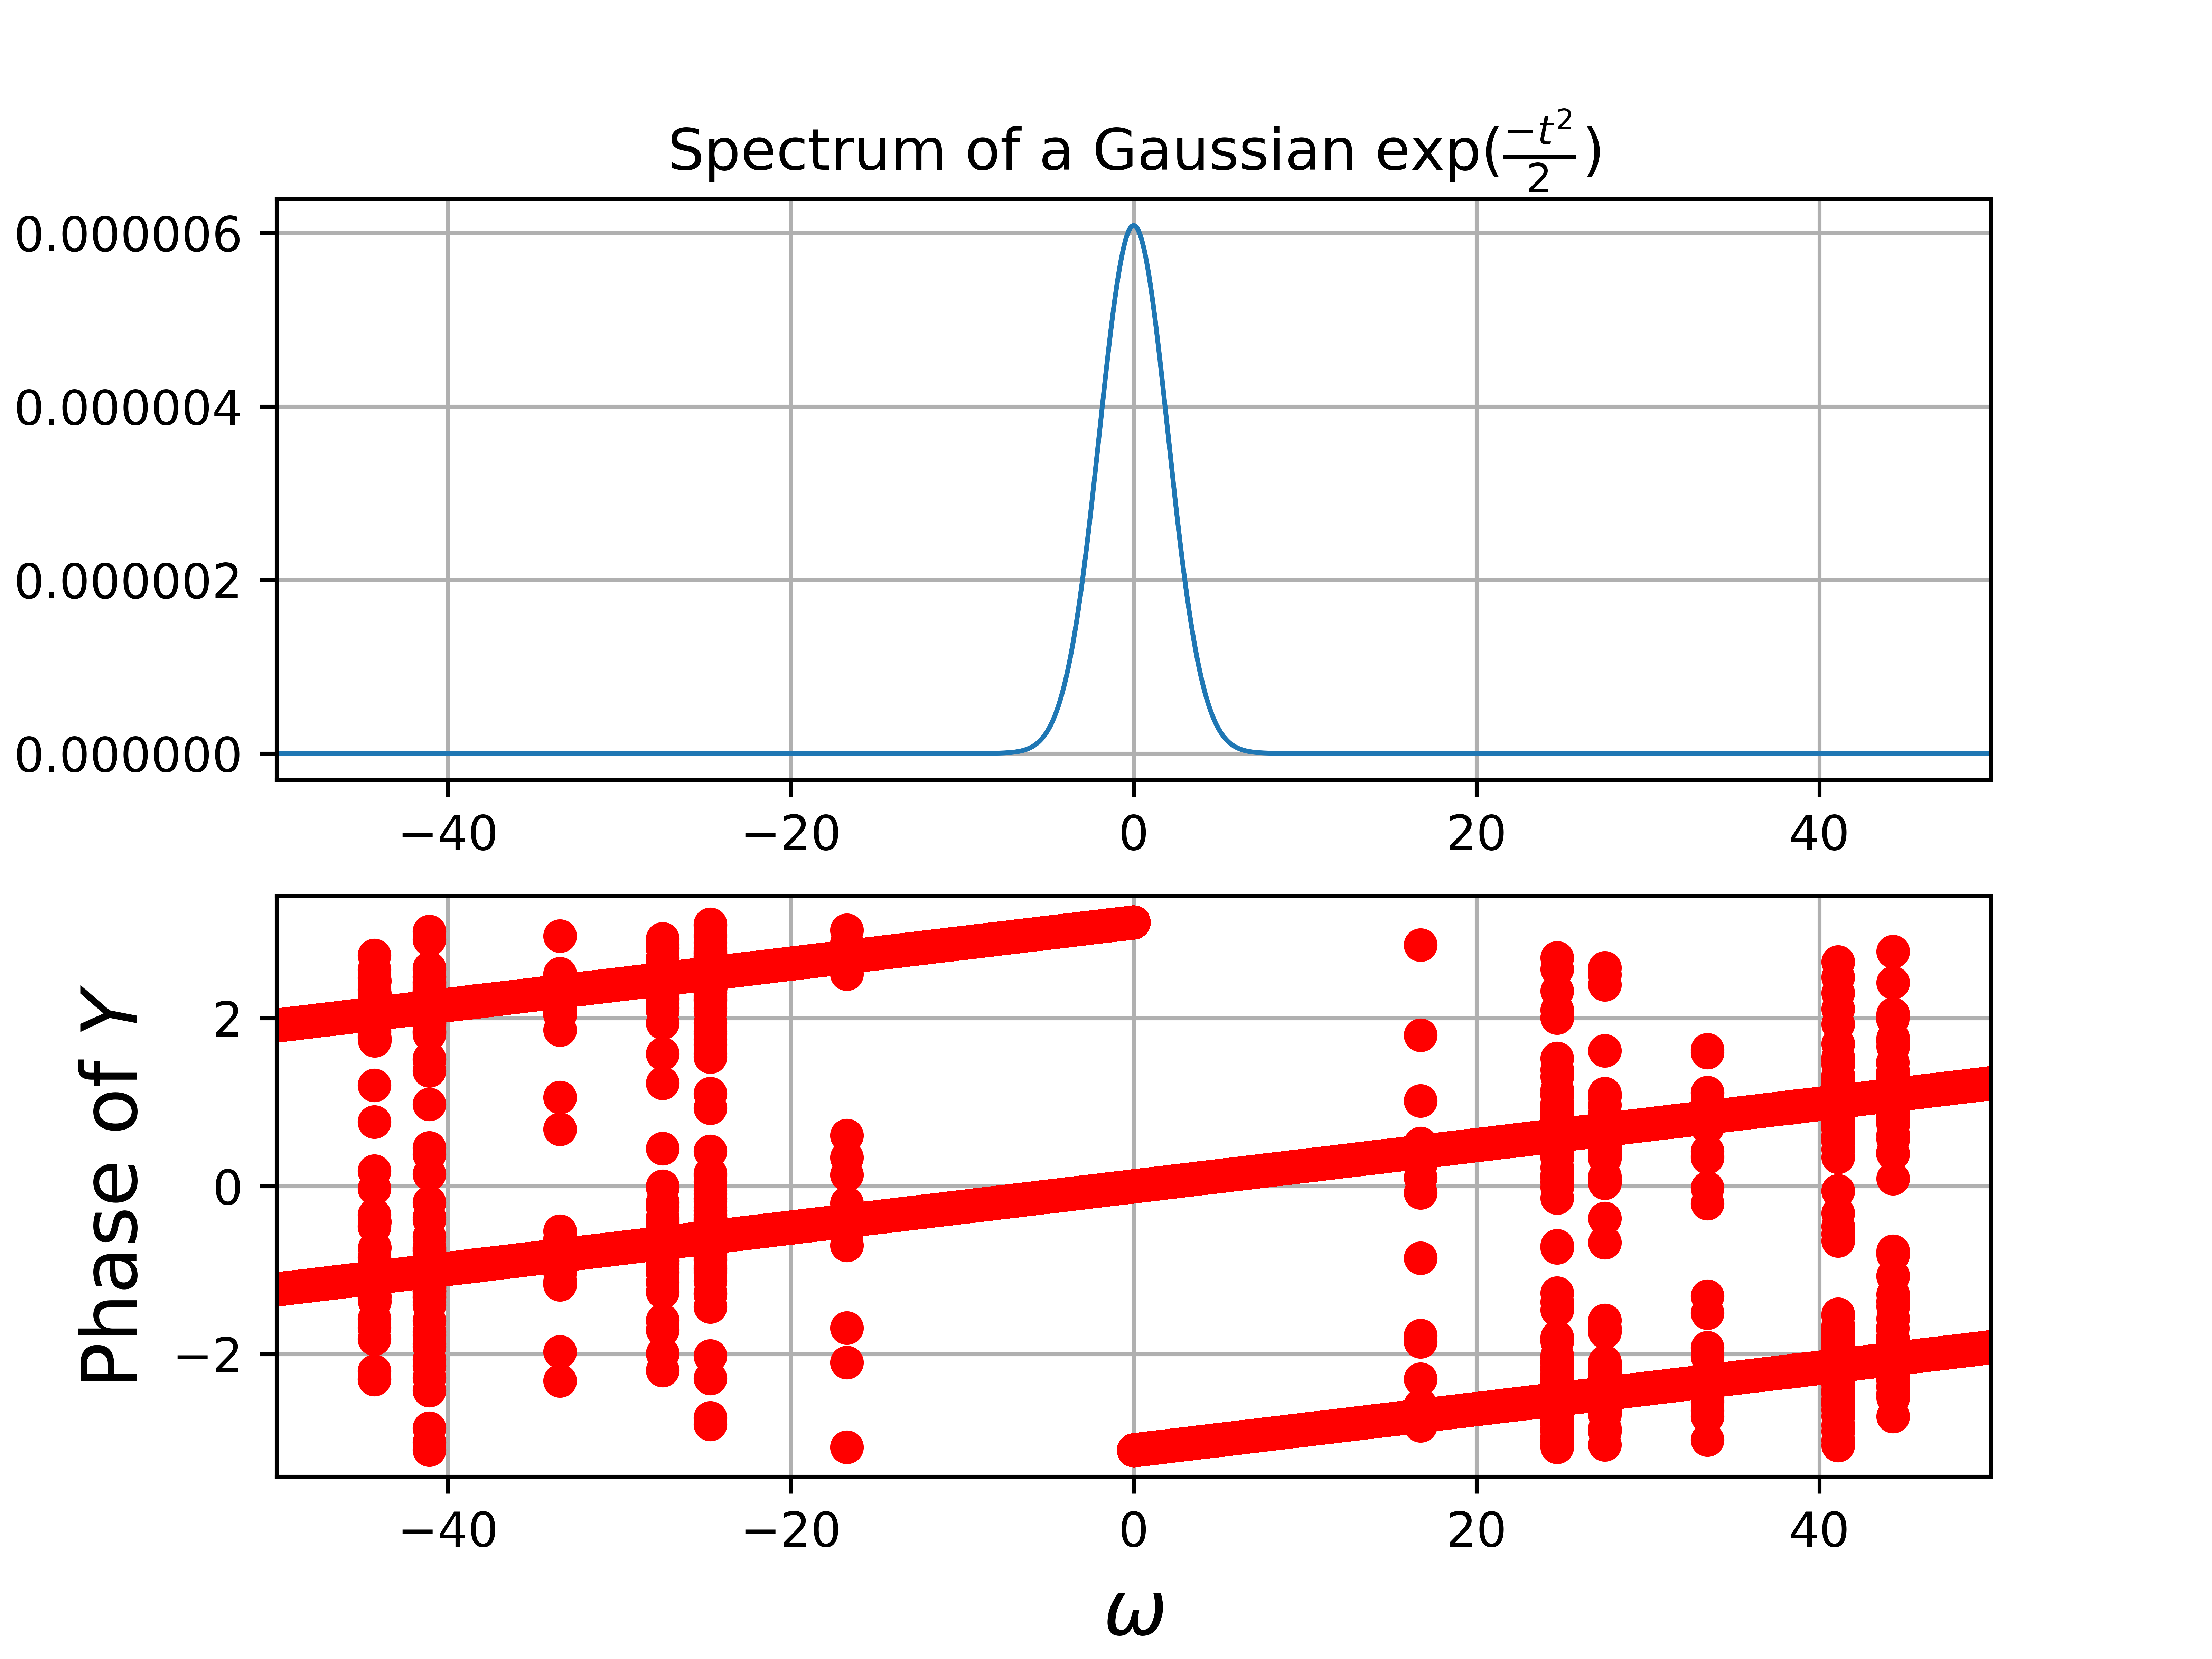
\includegraphics[scale=0.7]{images/fig9_forthelol.png}
    
    
    {Here just 2049 time samples used, but negative values still present in DFT}
    
    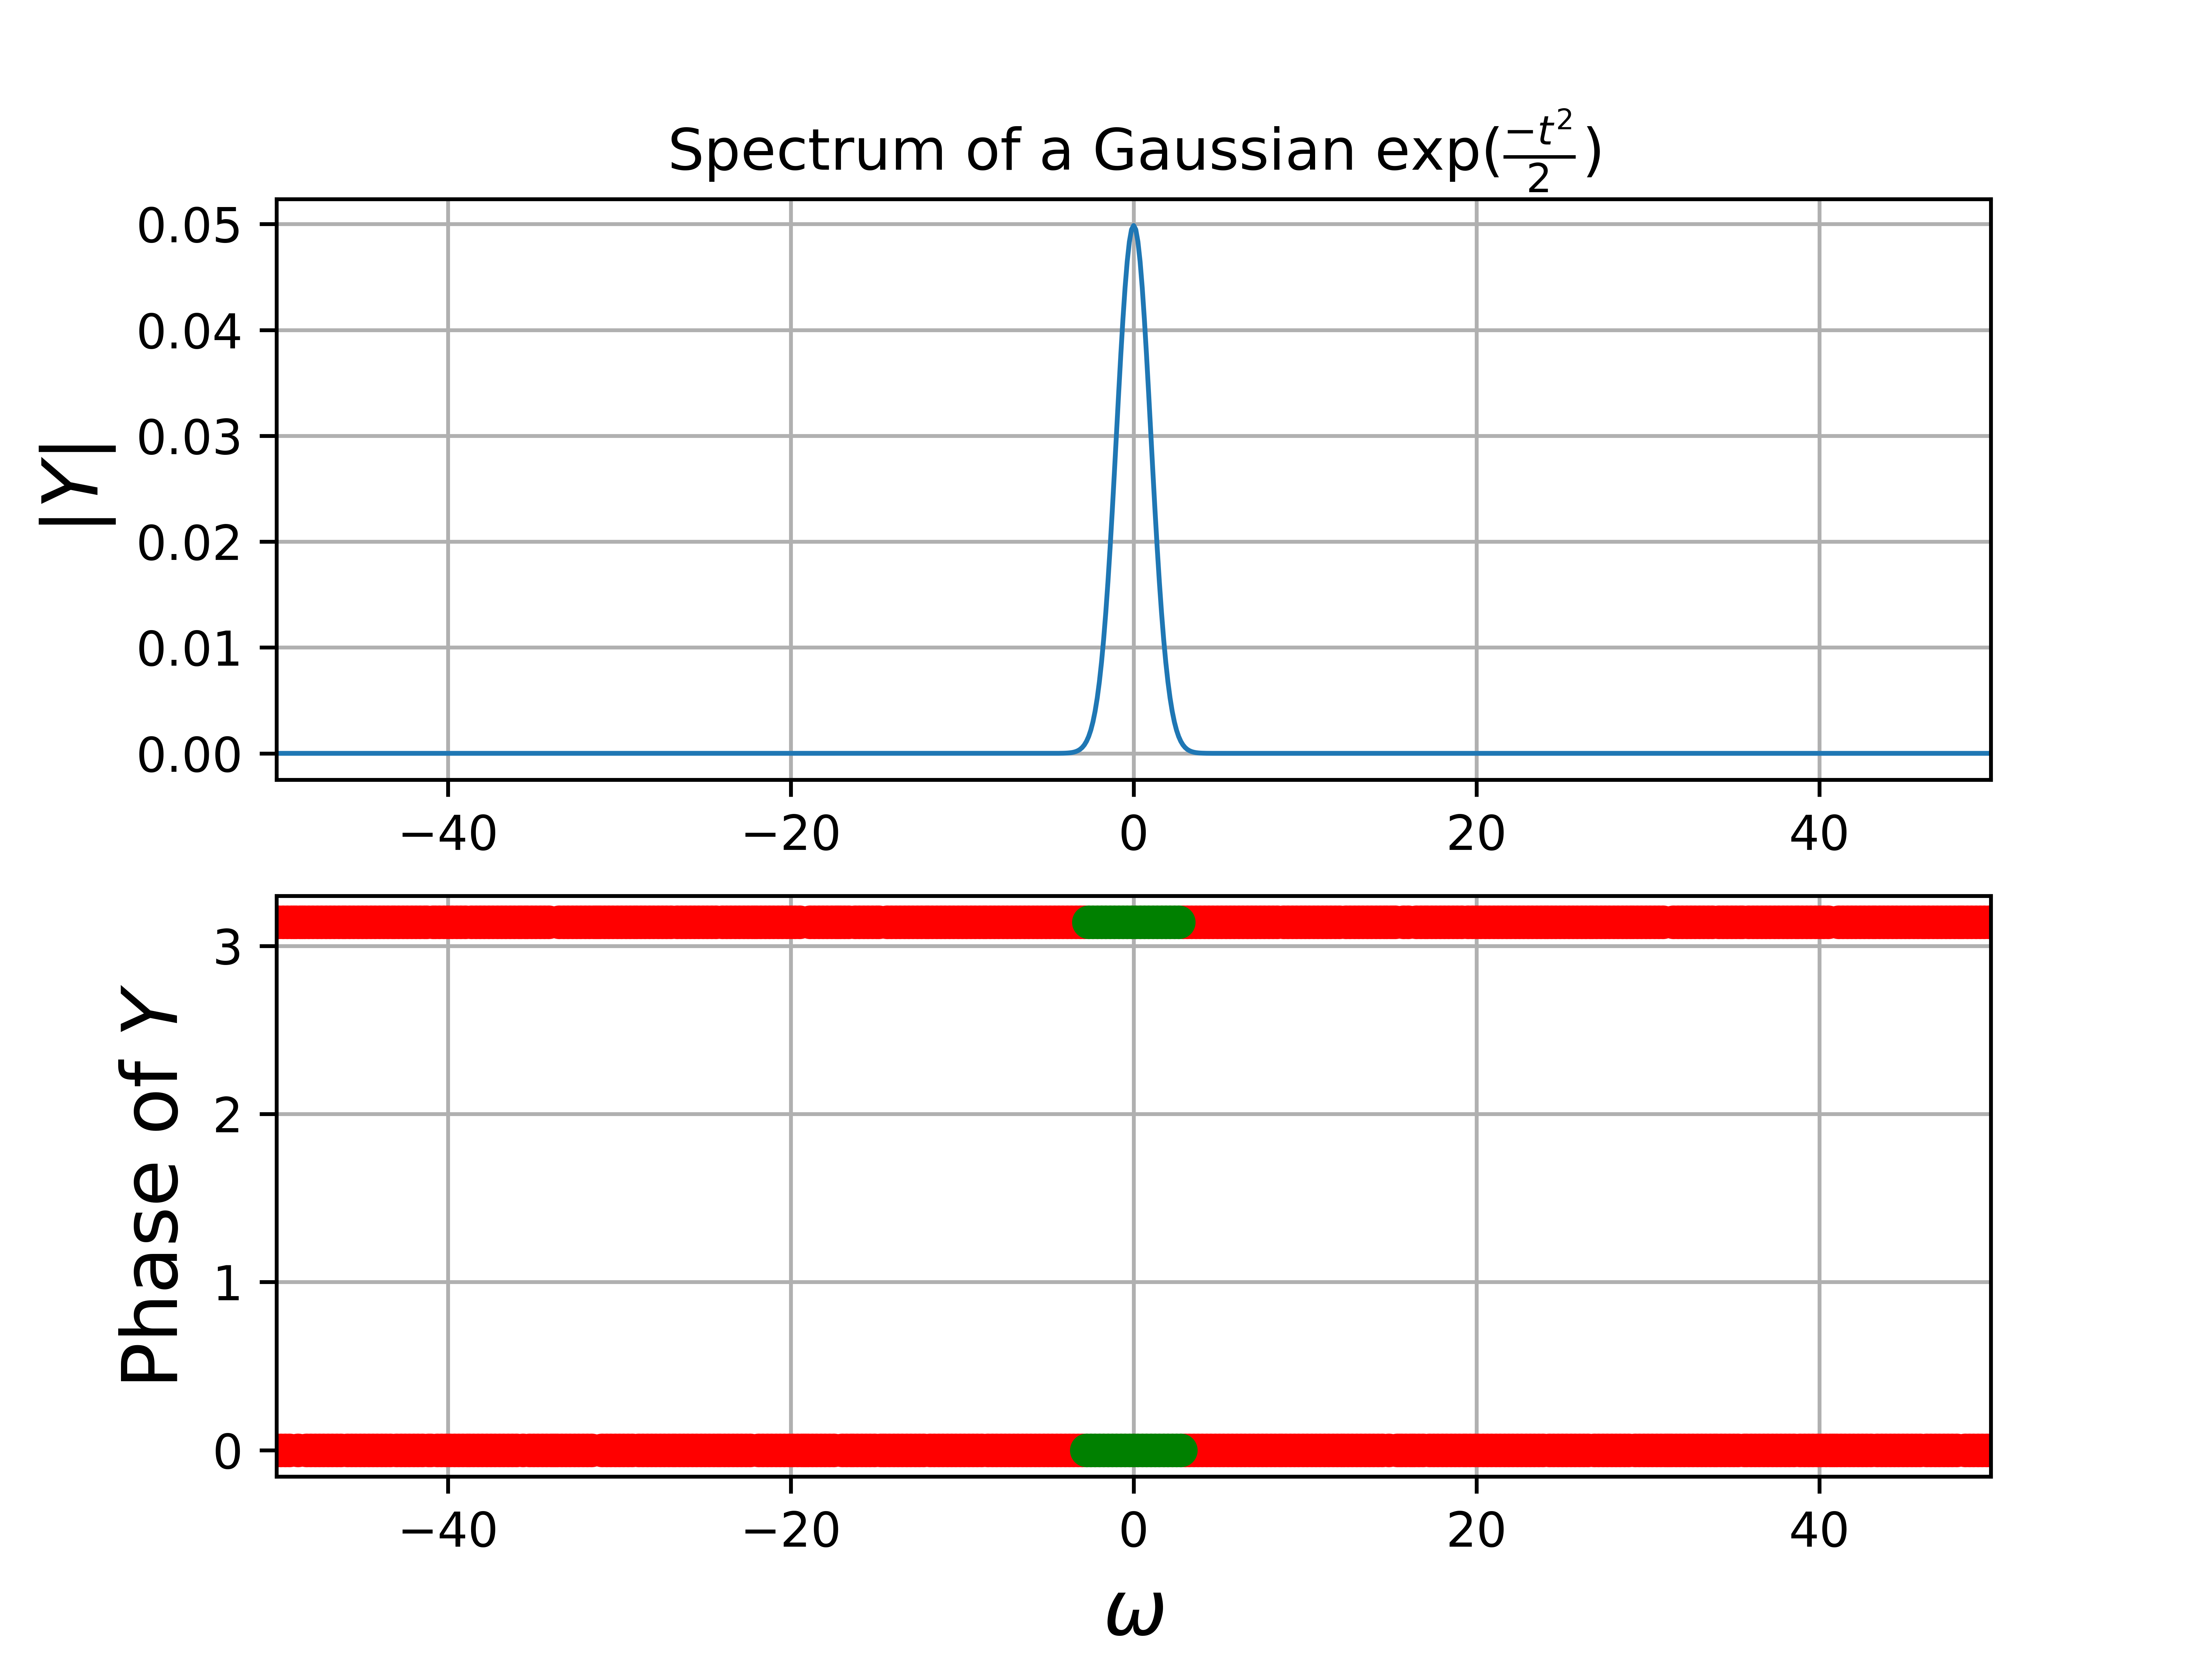
\includegraphics[scale=0.7]{images/fig10.png}
\end{center}
\pagebreak
Hence, we need to take the absolute value of the FFT and only then does it give the right graph as per the CFT.

For this, I couldn't use my helper function and had to write all the plotting commands separately.

Time was sampled over $[-8\pi,8\pi]$ and 4194305 samples were used. ($2^22 + 1$ samples).

The frequency was sampled over $[-262144,262144]$ ($262144 = \frac{4194304}{16}$)

\textbf{Code:}
\begin{lstlisting}[language=Python]
### We will be using 4194305 samples over -8pi to 8pi to get an error value less than 1e-6
t = np.linspace(-8*np.pi,8*np.pi,4194305)
y = np.exp(-(t**2)/2)
Y_init = np.fft.fftshift(abs(np.fft.fft(y)))/4194305
# Normalized value of Y
Y = Y_init*np.sqrt(2*np.pi)/max(Y_init)
w = np.linspace(-262144,262144,4194305)

Y_actual = np.sqrt(2*np.pi)*np.exp((-w**2)/2)

print("Error in Gaussian = "+str(max(abs(Y_actual-Y))))
plt.figure(9)
plt.subplot(2,1,1)
plt.plot(w,abs(Y),lw=1)
plt.xlim([-50,50])
plt.ylabel(r"$|Y|$",size=16)
plt.title(r"Spectrum of a Gaussian $\exp(\frac{-t^2}{2})$")
plt.grid(True)
plt.subplot(2,1,2)
plt.plot(w,np.angle(Y),'ro',lw=1)
ii = np.where(abs(Y)>1e-3)
plt.plot(w[ii],np.angle(Y[ii]),'go',lw=1)
plt.xlim([-50,50])
plt.ylabel(r"Phase of $Y$",size=16)
plt.xlabel(r"$\omega$",size=16)
plt.grid(True)
plt.savefig("images/fig9.png",dpi=1000)
plt.show()
\end{lstlisting}

The error in the Gaussian came out to be:

\texttt{Error in Gaussian = 4.390271375331878e-07}

And the plot was as follows:

\begin{center}
    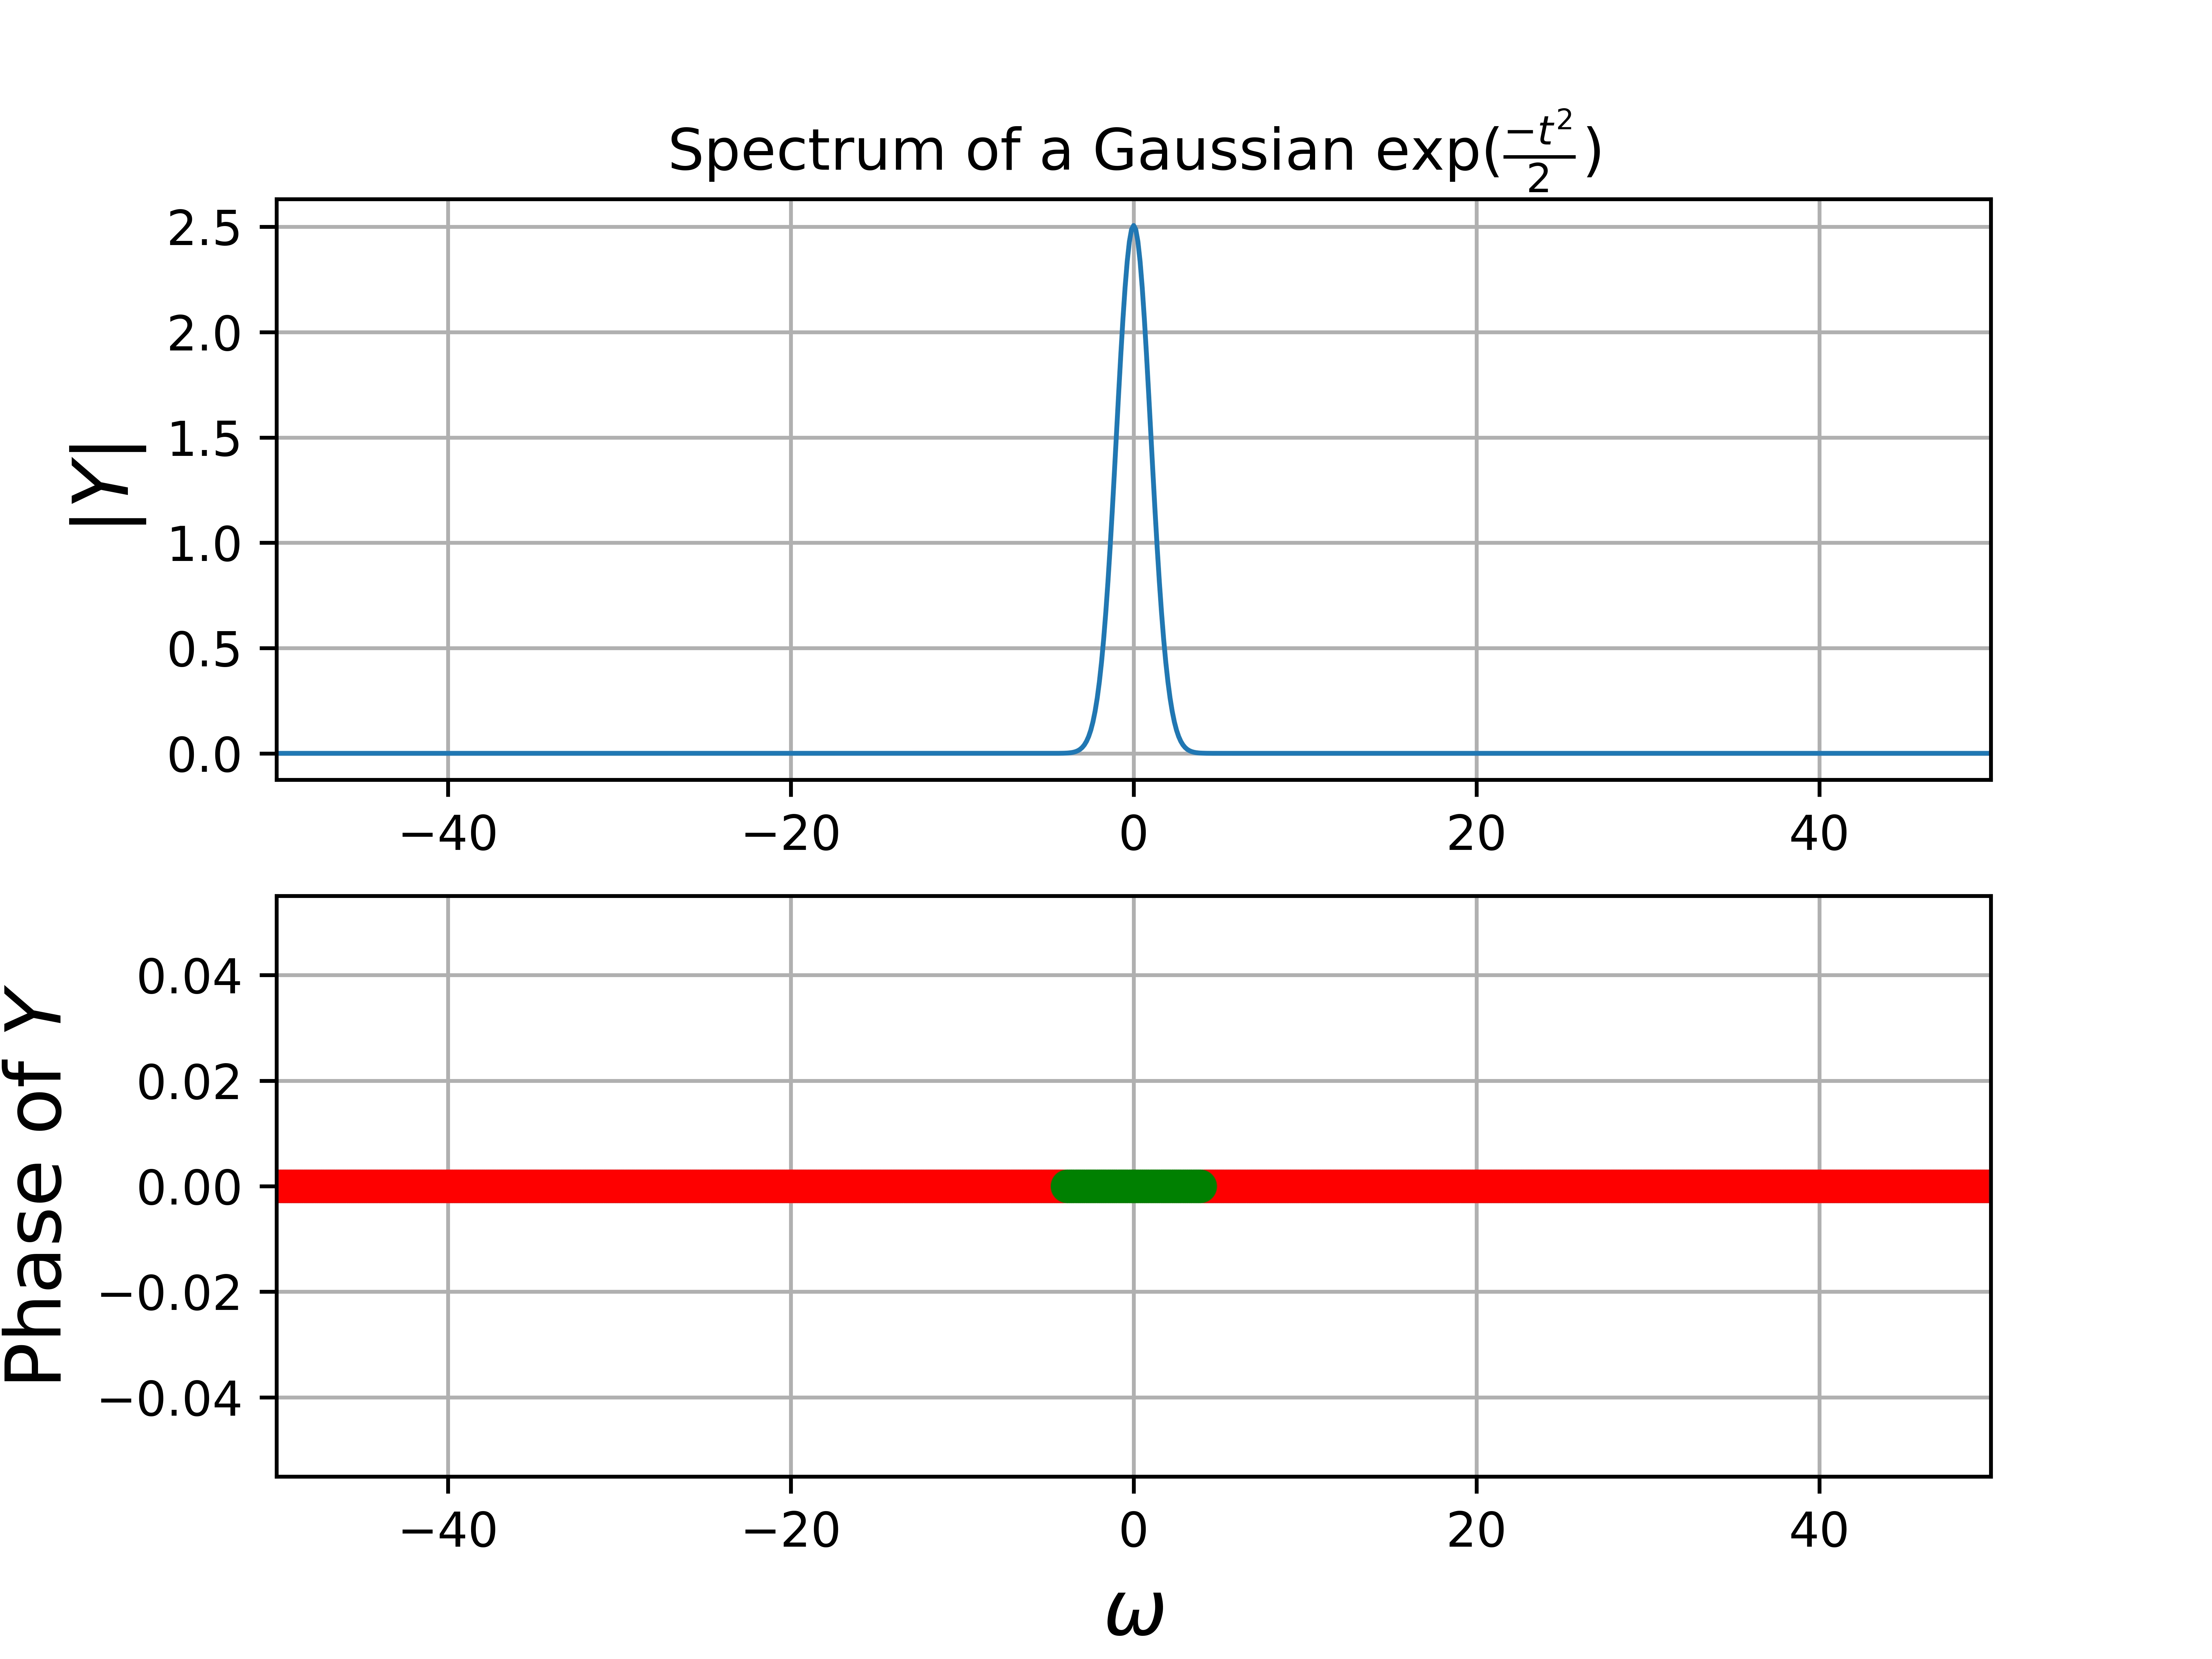
\includegraphics[scale=1]{images/fig9.png}
\end{center}

It can be observed that as we increase the number of samples, the Gaussian broadens.

\pagebreak
\section{Conclusions}
We analyzed the Fourier Transform of AM and FM waves.

The DFT of the AM wave contained impulses at carrier frequency $\pm$ side band frequency.

The DFT of an FM wave contained infinite impulses which died out as we moved away from the carrier frequency.

The DFT of a Gaussian input was a Gaussian as well, but unless the input time samples are centered at zero, the output doesn't come out the same as the CFT of a Gaussian.

However, with some minor tweaking, it was possible to convert it into the right form.

Overall, the \texttt{fft} toolkit in NumPy was found to be extremely useful and easy to use, although the plotting took more effort than usual due to having both phase and magnitude plots in each of the spectra.

\end{document}